\chapter{Design}
This chapter provides a representation of efforts one must face to make a jump from dry theoretical models to a virtually real product.

\section{On a quest to perfect parameters}
Our journey begins with a necessity to define restrictions of the problem. The intended environment would be a 4K cryogenic chamber (figure \ref{fig:4K_chamber}), which imposes dimensions restrictions. The ion trap requires a defined frequency for successful confinement of ions and has a capacitance. Summarized restrictions can be found in table \ref{tbl:restrictions}.

\begin{table}[h]
\centering
\begin{tabular}{| l | r | r |}
	\hline
	Parameter & Description & Value \\
	\hline \hline
	&&\\[-1em]
	$V_{max}$ & Maximum volume of the resonator & $\left( 60\text{ mm} \right)^3$ \\[5pt]
	\hline
	$\omega_0$ & Target frequency of the trap & 40 MHz \\
	\hline
	$C_{trap}$ & Capacitance of the trap & 10--20 pF \\
	\hline
\end{tabular}	
\caption{Restrictions of a system}
\label{tbl:restrictions}
\end{table}

\subsection{First iteration}
Siverns' model \cite{Siverns2012} is dependent on outcomes from Macalpine's model \cite{Macalpine2000} thus one needs to find these beforehand. Exact value of a trap's capacitance is unknown at the moment of calculations so it was decided to use and compare values from a following set of capacitances: $C_{trap} = [10, 15, 20]\text{ pF}$. The modified Macalpine's model, found in the appendix \ref{chapter:macalpine_code}, also predicts resonant frequency shift when connecting a capacitor. The unloaded frequency needed to be varied until the loaded frequency equals target frequency. Results are provided in table \ref{tbl:macalpine}, naming is consistent with \cite{Macalpine2000}.

\begin{table}[h]
\centering
\begin{tabular}{| l | r | r | r |}
	\hline
	Parameter & \multicolumn{3}{r |}{Value} \\
	\hline \hline
	$C_{trap}$, pF & 10 & 15 & 20 \\
	\hline
	$B$, mm (length of a shield) & \multicolumn{3}{r |}{60.0} \\
	\hline
	$D$, mm (diameter of a shield) & \multicolumn{3}{r |}{45.0} \\
	\hline
	$b$, mm (length of a coil) & \multicolumn{3}{r |}{37.1} \\
	\hline
	$N_{t}$ (number of turns) & 11.0 & 9.2 & 8.1 \\
	\hline
	$d_0$, mm (diameter of a wire) & 1.7 & 2.0 & 2.3 \\
	\hline
	$\tau$, mm (pitch of a helix) & 3.4 & 4.0 & 4.6 \\
	\hline
	$f_0$, MHz (unloaded frequency) & 97.0 & 116.0 & 132.8 \\
	\hline
	$Q$ (unloaded quality factor) & 873.2 & 954.8 & 1022.4 \\
	\hline
\end{tabular}
\caption{Joint output of the appendix \ref{chapter:macalpine_code}}
\label{tbl:macalpine}
\end{table}

\subsection{Precise fit}
After defining an approximate region of interest we can proceed to calculations utilizing Siverns' model \cite{Siverns2012} with implementation provided in the appendix \ref{chapter:siverns_code}. Volume requirements were also better clarified with the goal to get the best quality factor by varying coil's parameters. Updated restrictions can be found in the table \ref{tbl:restrictions_siverns}. One could argue that all values of $d_0$ are lower than the recommended in \cite{Siverns2012} thickness of 5 mm. This is true and additional measures to handle it can be found in section \ref{subsection:helix_support}.

\begin{table}[h]
\centering
\begin{tabular}{| l | r | r | r |}
	\hline
	Parameter & \multicolumn{3}{r |}{Value} \\
	\hline \hline
	$C_{trap}$, pF & 10 & 15 & 20 \\
	\hline
	$B$, mm (length of a shield) & \multicolumn{3}{r |}{56.0} \\
	\hline
	$D_{max}$, mm (max diameter of a shield) & \multicolumn{3}{r |}{38.0} \\
	\hline
	$d_0$, mm (diameter of a wire) & 1.7 & 2.0 & 2.3 \\
	\hline
	$\tau$, mm (pitch of a helix) & 3.4 & 4.0 & 4.6 \\
	\hline
\end{tabular}
\caption{Restrictions for the Siverns' model}
\label{tbl:restrictions_siverns}
\end{table}

Fixed values of the table \ref{tbl:restrictions_siverns} allow us to independently change 2 remaining parameters --- diameter of a shield and diameter of a coil. Appendix's \ref{chapter:siverns_code} output of $Q$ values is provided in the figures \ref{fig:q_plot_10}, \ref{fig:q_plot_15}, \ref{fig:q_plot_20}. By selecting a point in a $\{d, \gamma = d / D\}$ space that maximizes $Q$ for a set of $C_{trap}$ values we get final parameters for our RF resonator as defined in the table \ref{tbl:final_parameters}.
\FloatBarrier
\begin{figure}[h!]
\centering
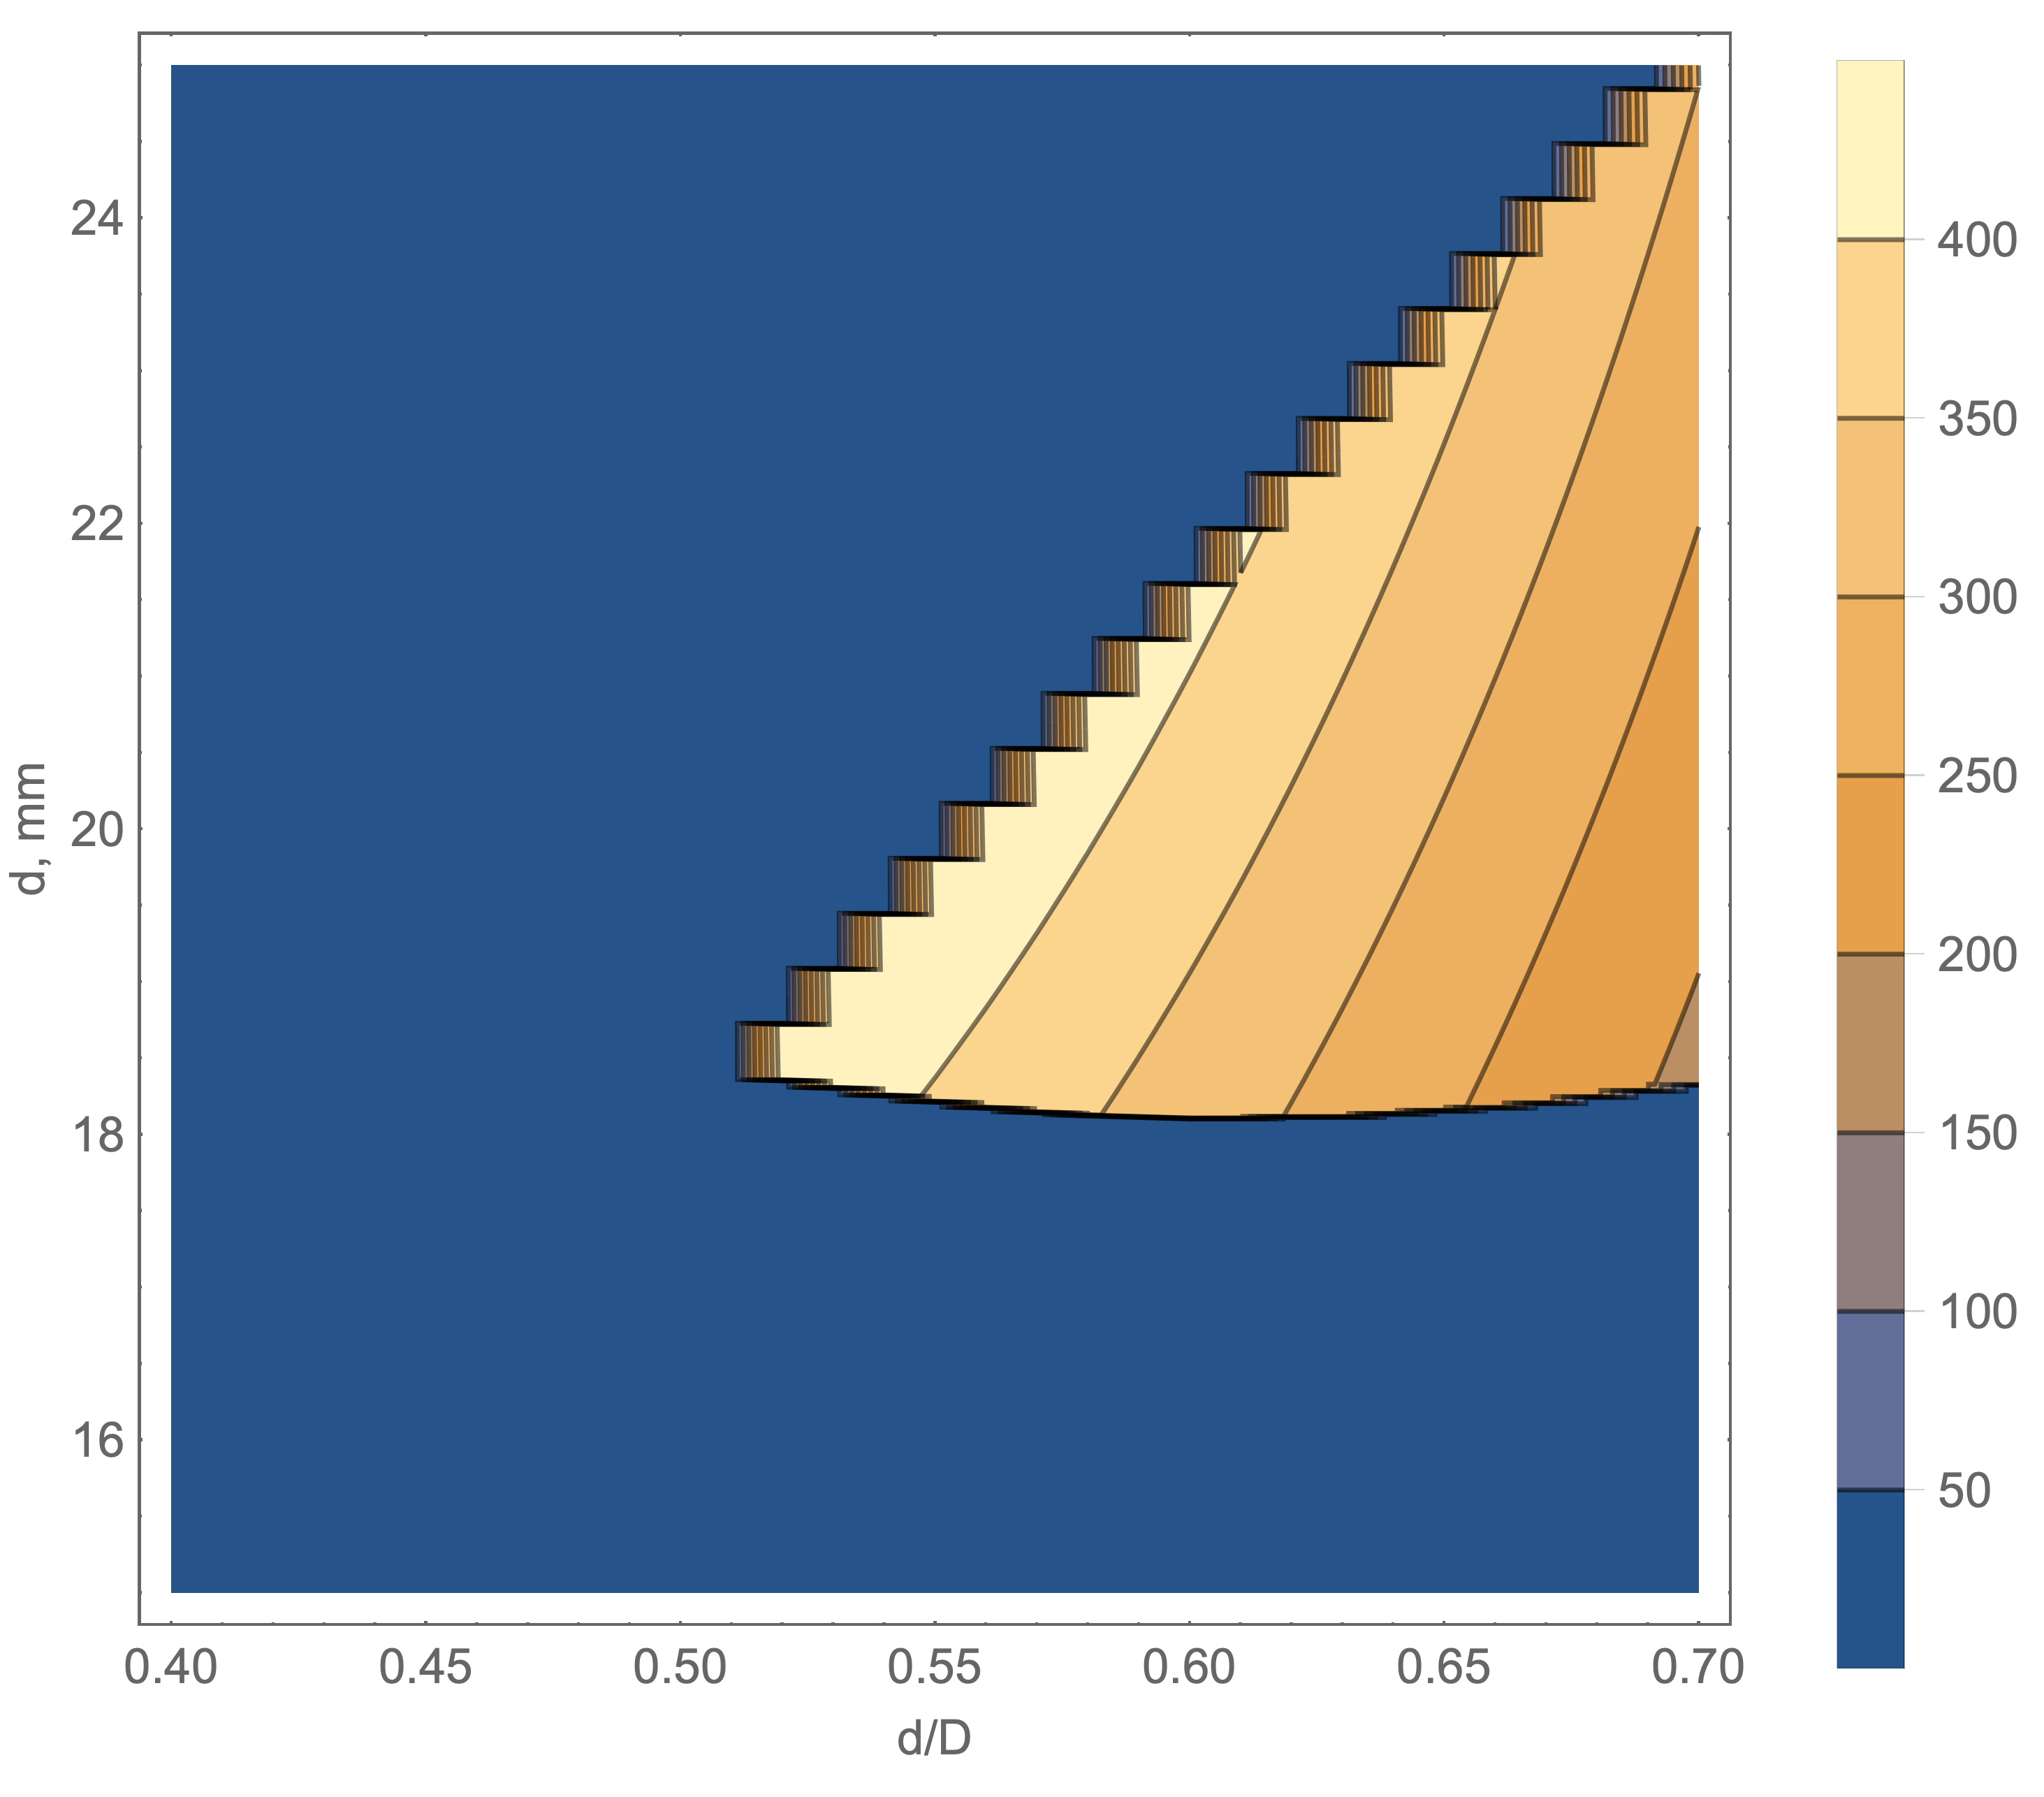
\includegraphics[width=.78\textwidth]{images/q_plot_siverns_tex_10}
\caption{$Q$ values plot for $C_{trap} = 10$ pF}
\label{fig:q_plot_10}
\end{figure}
\begin{figure}[h!]
\centering
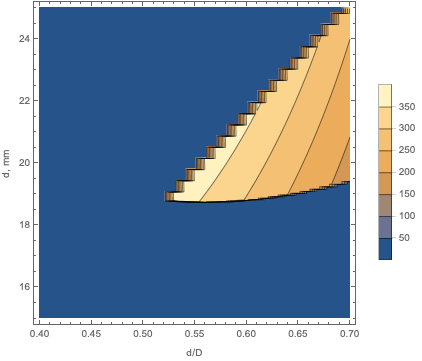
\includegraphics[width=.78\textwidth]{images/q_plot_siverns_tex_15}
\caption{$Q$ values plot for $C_{trap} = 15$ pF}
\label{fig:q_plot_15}
\end{figure}
\begin{figure}[h!]
\centering
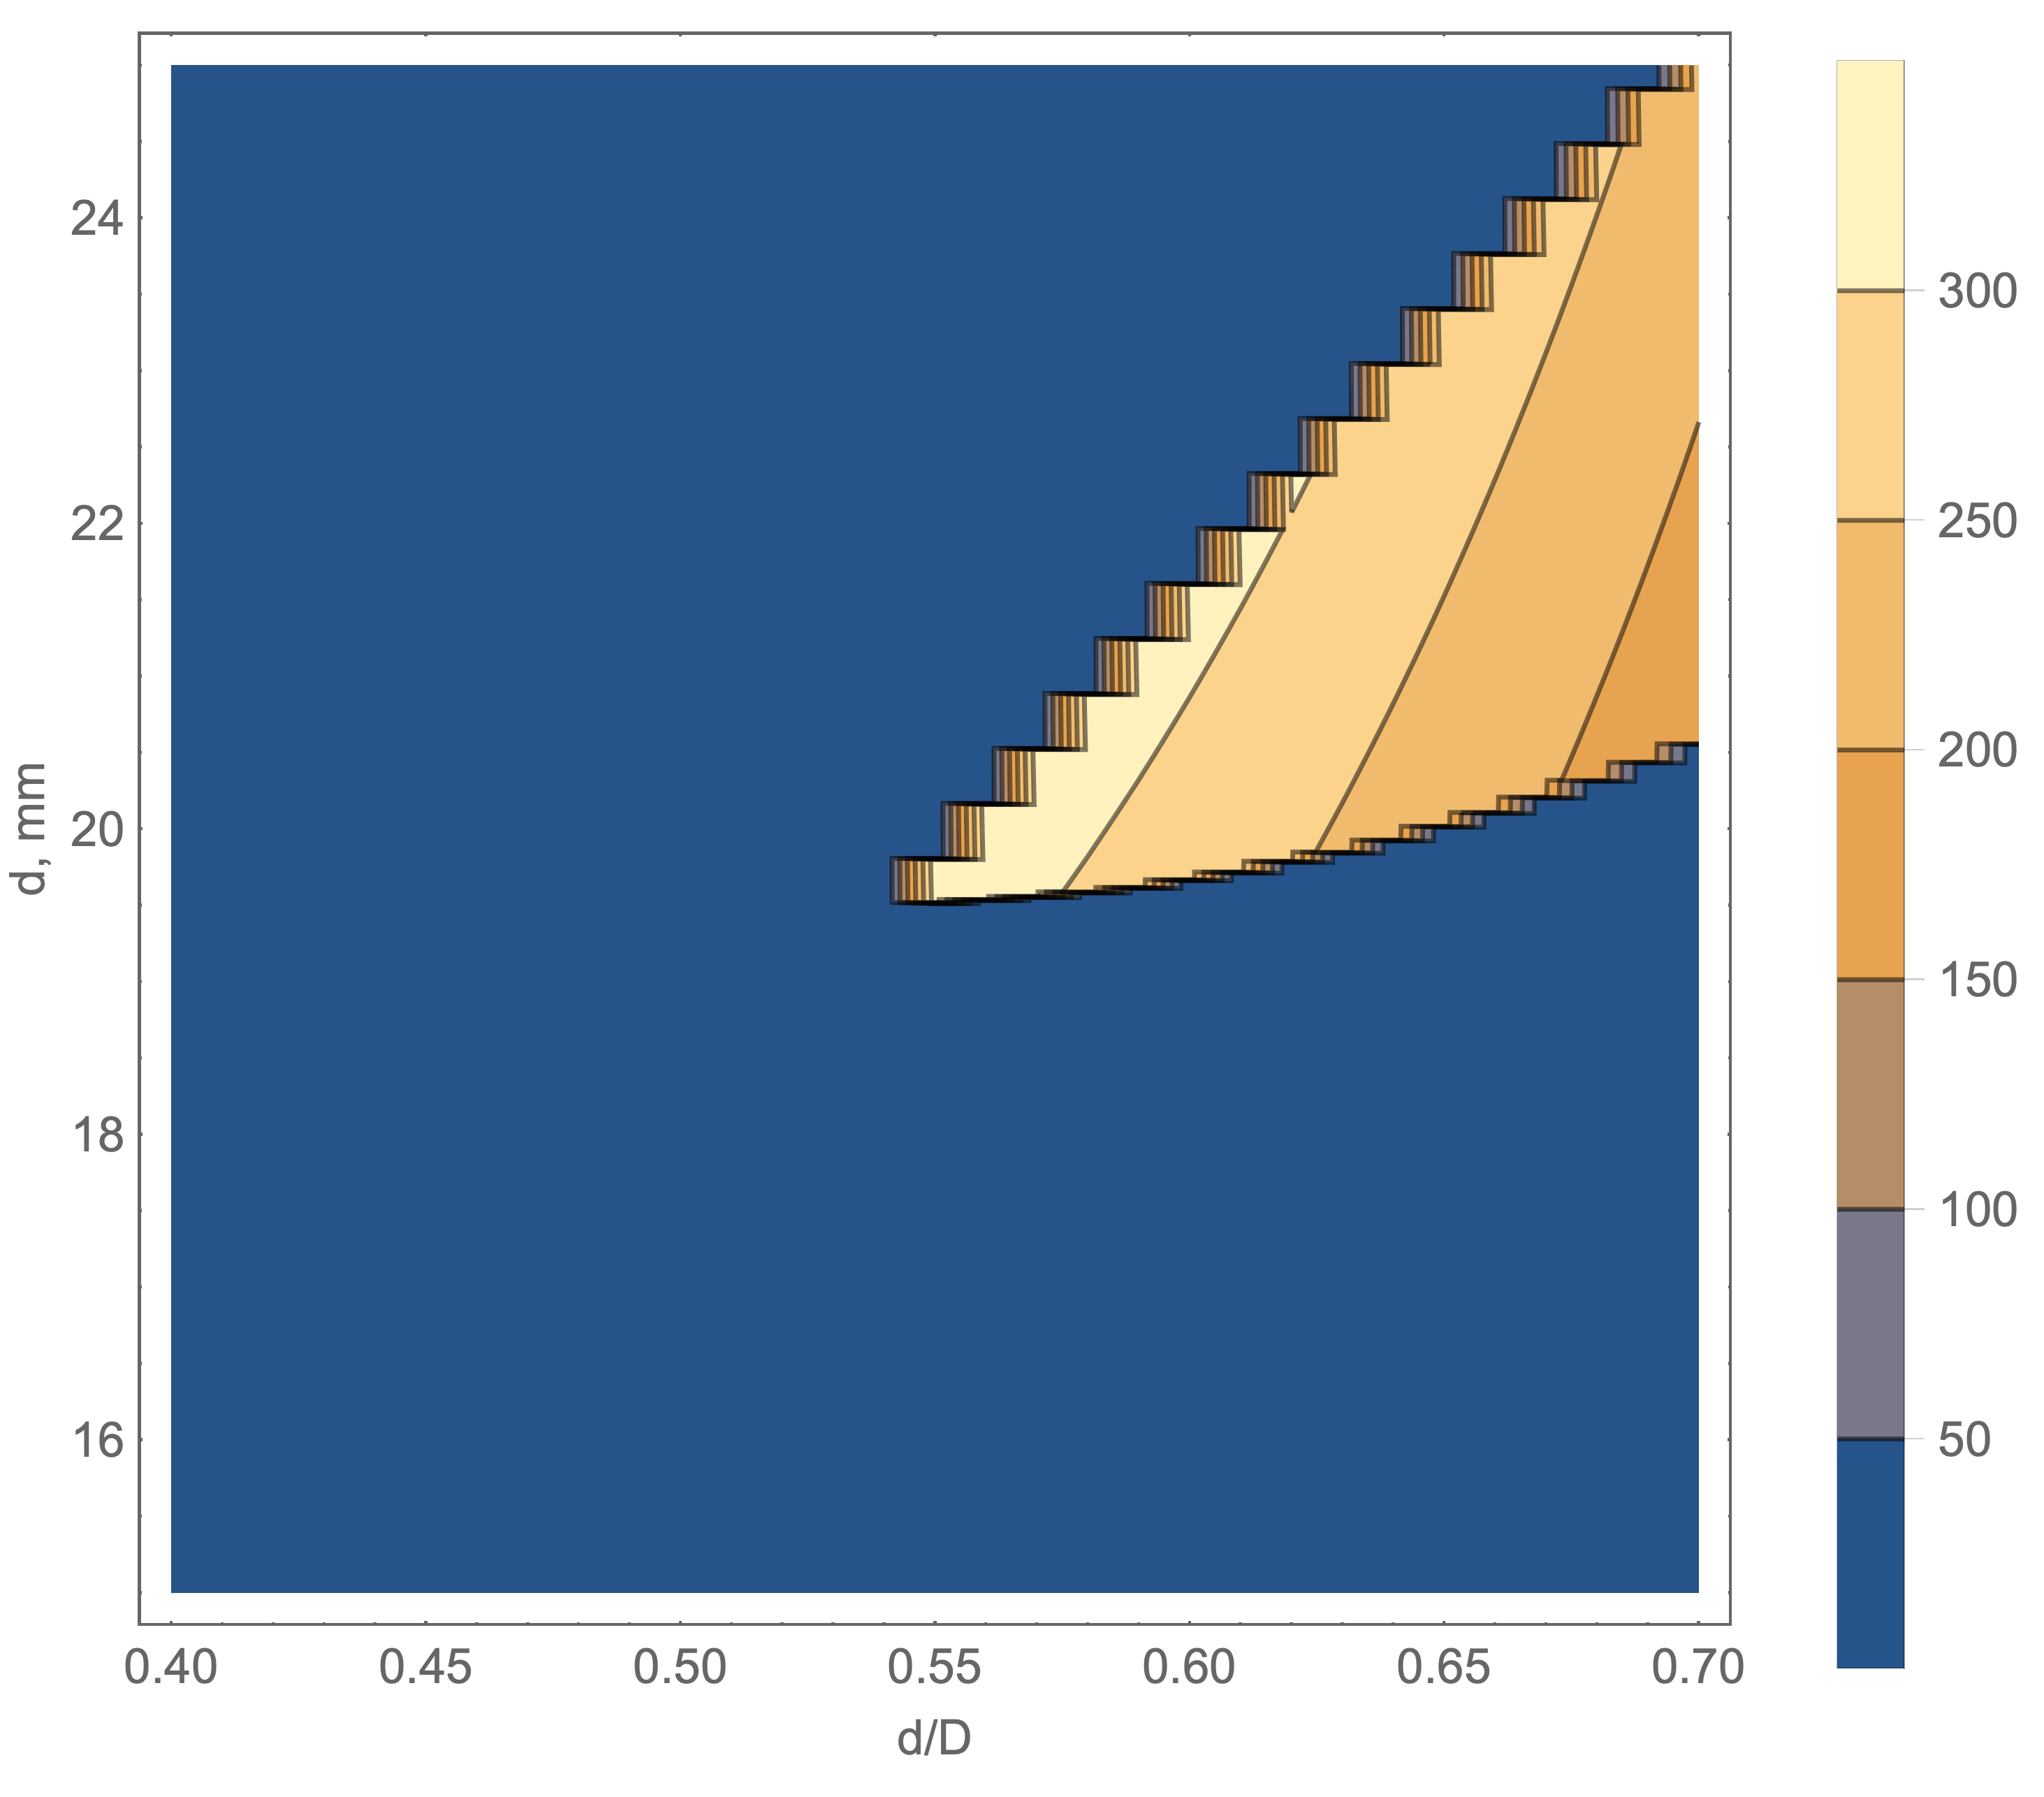
\includegraphics[width=.78\textwidth]{images/q_plot_siverns_tex_20}
\caption{$Q$ values plot for $C_{trap} = 20$ pF}
\label{fig:q_plot_20}
\end{figure}
\FloatBarrier
\begin{table}[h]
\centering
\begin{tabular}{| l | r |}
	\hline
	Parameter & Value\\
	\hline \hline
	$B$, mm (length of a shield) & 56.0 \\
	\hline
	$D$, mm (diameter of a shield) & 34.5 \\
	\hline
	$d$, mm (diameter of a coil) & 19.0 \\
	\hline
	$b$, mm (length of a coil) & 40.0 \\
	\hline
	$N_{t}$ (number of turns) & 10.0 \\
	\hline
	$d_0$, mm (diameter of a wire) & 2.0 \\
	\hline
	$\tau$, mm (pitch of a helix) & 4.0 \\
	\hline
\end{tabular}
\caption{Final parameters of an RF resonator}
\label{tbl:final_parameters}
\end{table}

\section{Shaping the 3D model}
With all dimensions in our hands we can start implementing them in a 3D design for the workshop. This section provides an overview of all parts used, their features and reasonings.

\clearpage
\subsection{RF resonator}
\label{subsection:rf_resonator_3d}
Assembly of the RF resonator is shown on the figure \ref{fig:resonator}. Every part is produced from oxygen-free copper. Colors are adjusted for a better perception.

\begin{figure}[h]
	\centering
	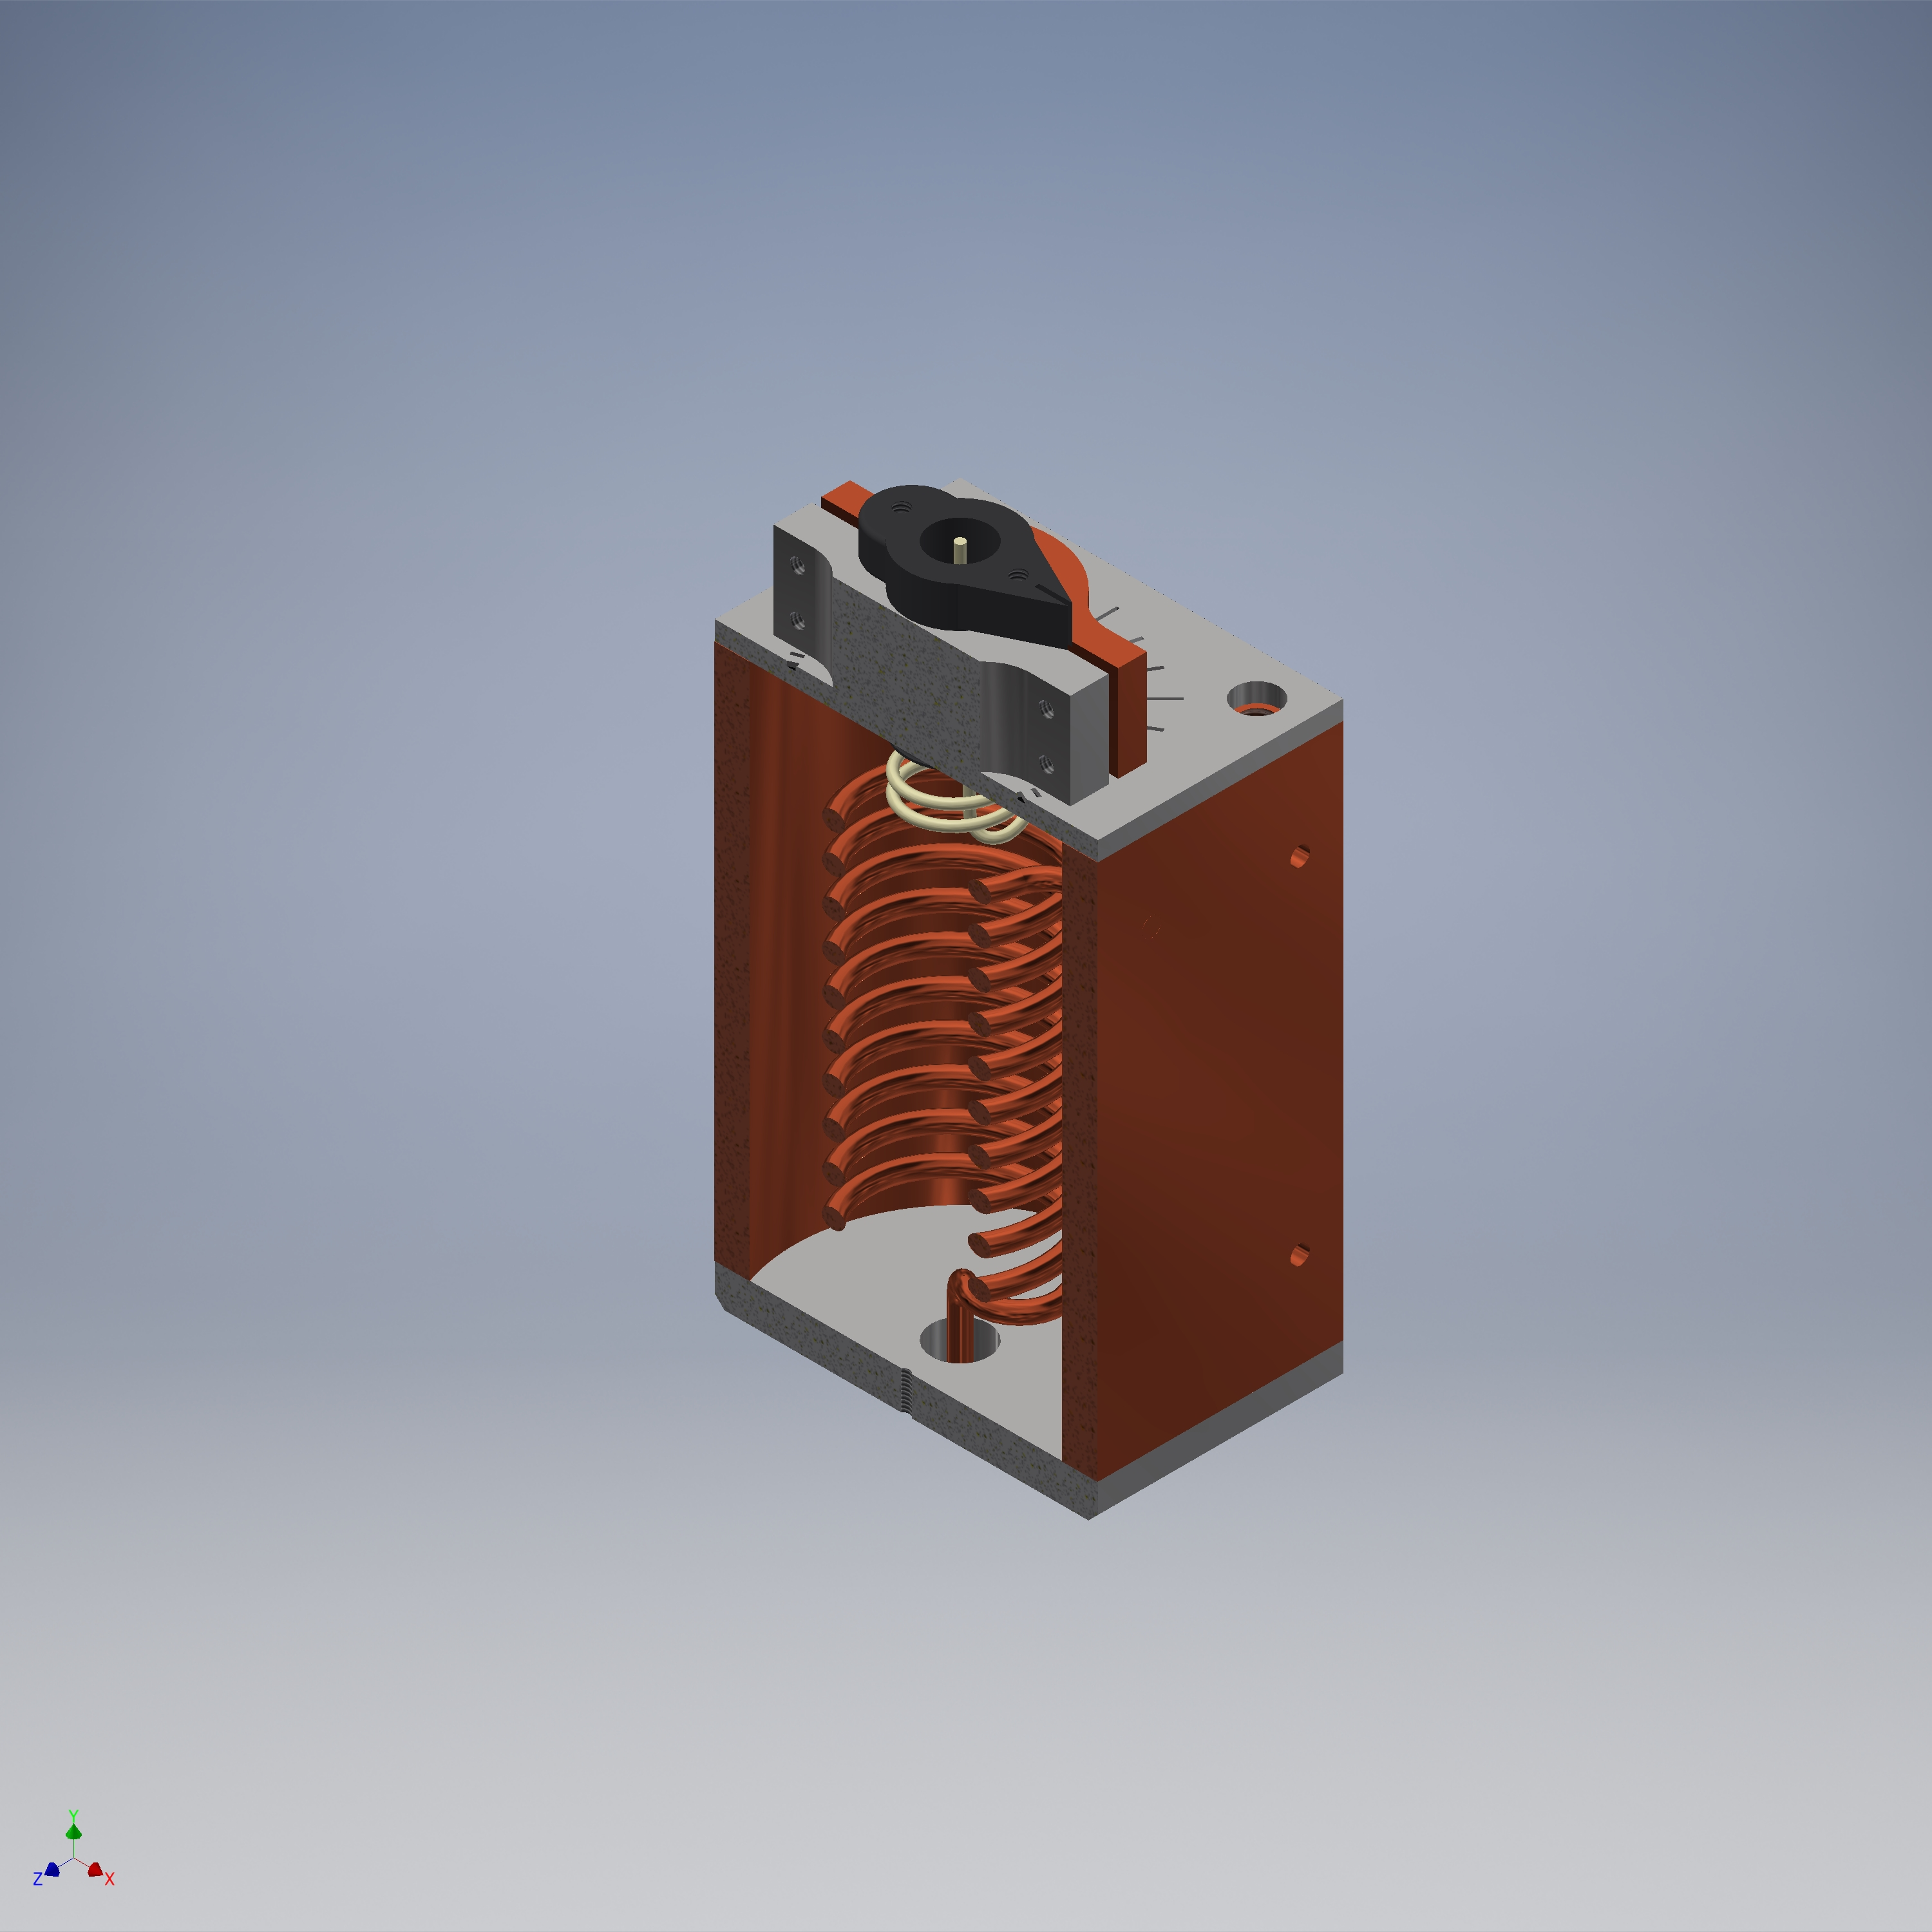
\includegraphics[width=\textwidth]{images/resonator}
	\caption{3D model of an RF resonator}
	\label{fig:resonator}
\end{figure}

\clearpage
\subsection{Bottom cap}
\label{subsection:cap_bottom}
Bottom cap as displayed in the figure \ref{fig:cap_bottom} features:
\begin{itemize}
	\item output hole for the helix (\ref{subsection:helix})
	\item 4xM4 clearance holes to connect to the shield (\ref{subsection:shield})
	\item 2xM2 thread holes for a SMA connector for the helix (\ref{subsection:helix})
\end{itemize}

\begin{figure}[h]
	\centering
	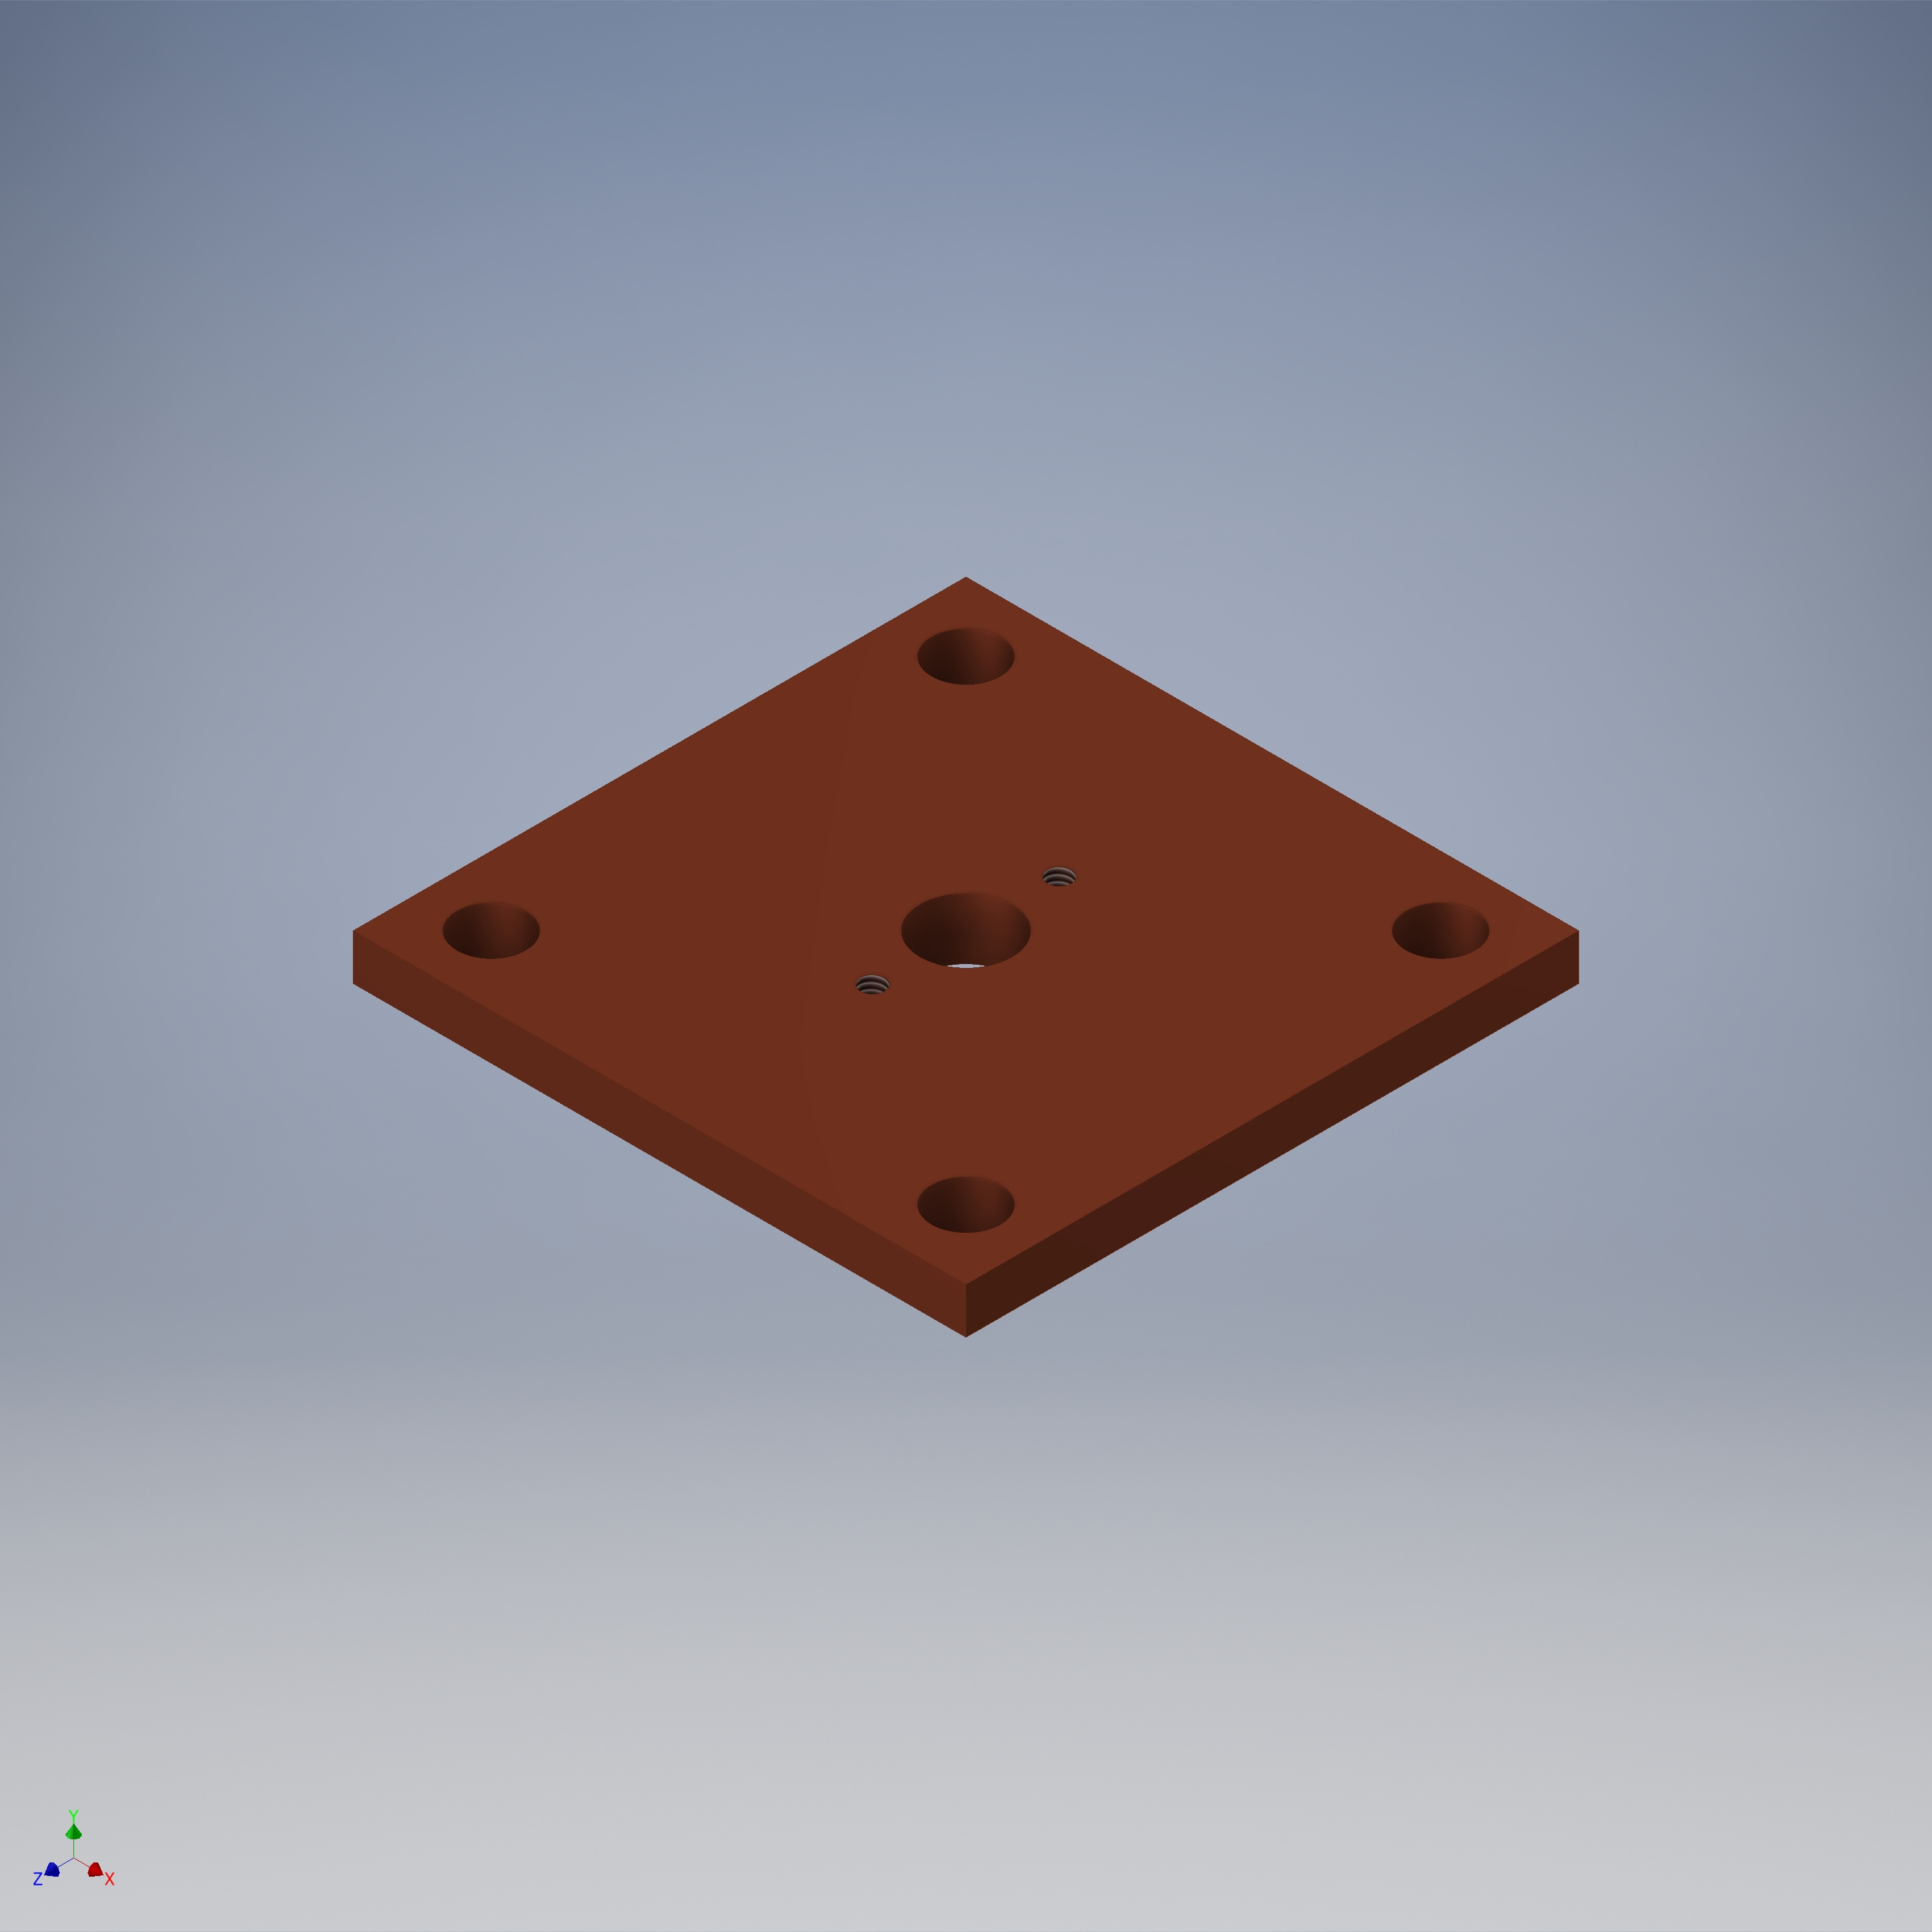
\includegraphics[width=\textwidth]{images/cap_bottom}
	\caption{3D model of a bottom cap}
	\label{fig:cap_bottom}
\end{figure}

\clearpage
\subsection{Shield}
\label{subsection:shield}
Shield as displayed in the figure \ref{fig:shield} features:
\begin{itemize}
	\item 4xM4 thread holes to connect to the top cap (\ref{subsection:cap_top})
	\item 4xM4 thread holes to connect to the 4K chamber (figure \ref{fig:4K_chamber})
	\item 4xM4 thread holes to connect to the bottom cap (\ref{subsection:cap_bottom})
	\item 12x ventilation holes for M4 thread holes to avoid the slow leakage of the remaining air between the screw and the shield into the vacuum of the cryostat	
	\item hole for the helix connection (\ref{subsection:helix})
\end{itemize}

\begin{figure}[h]
	\centering
	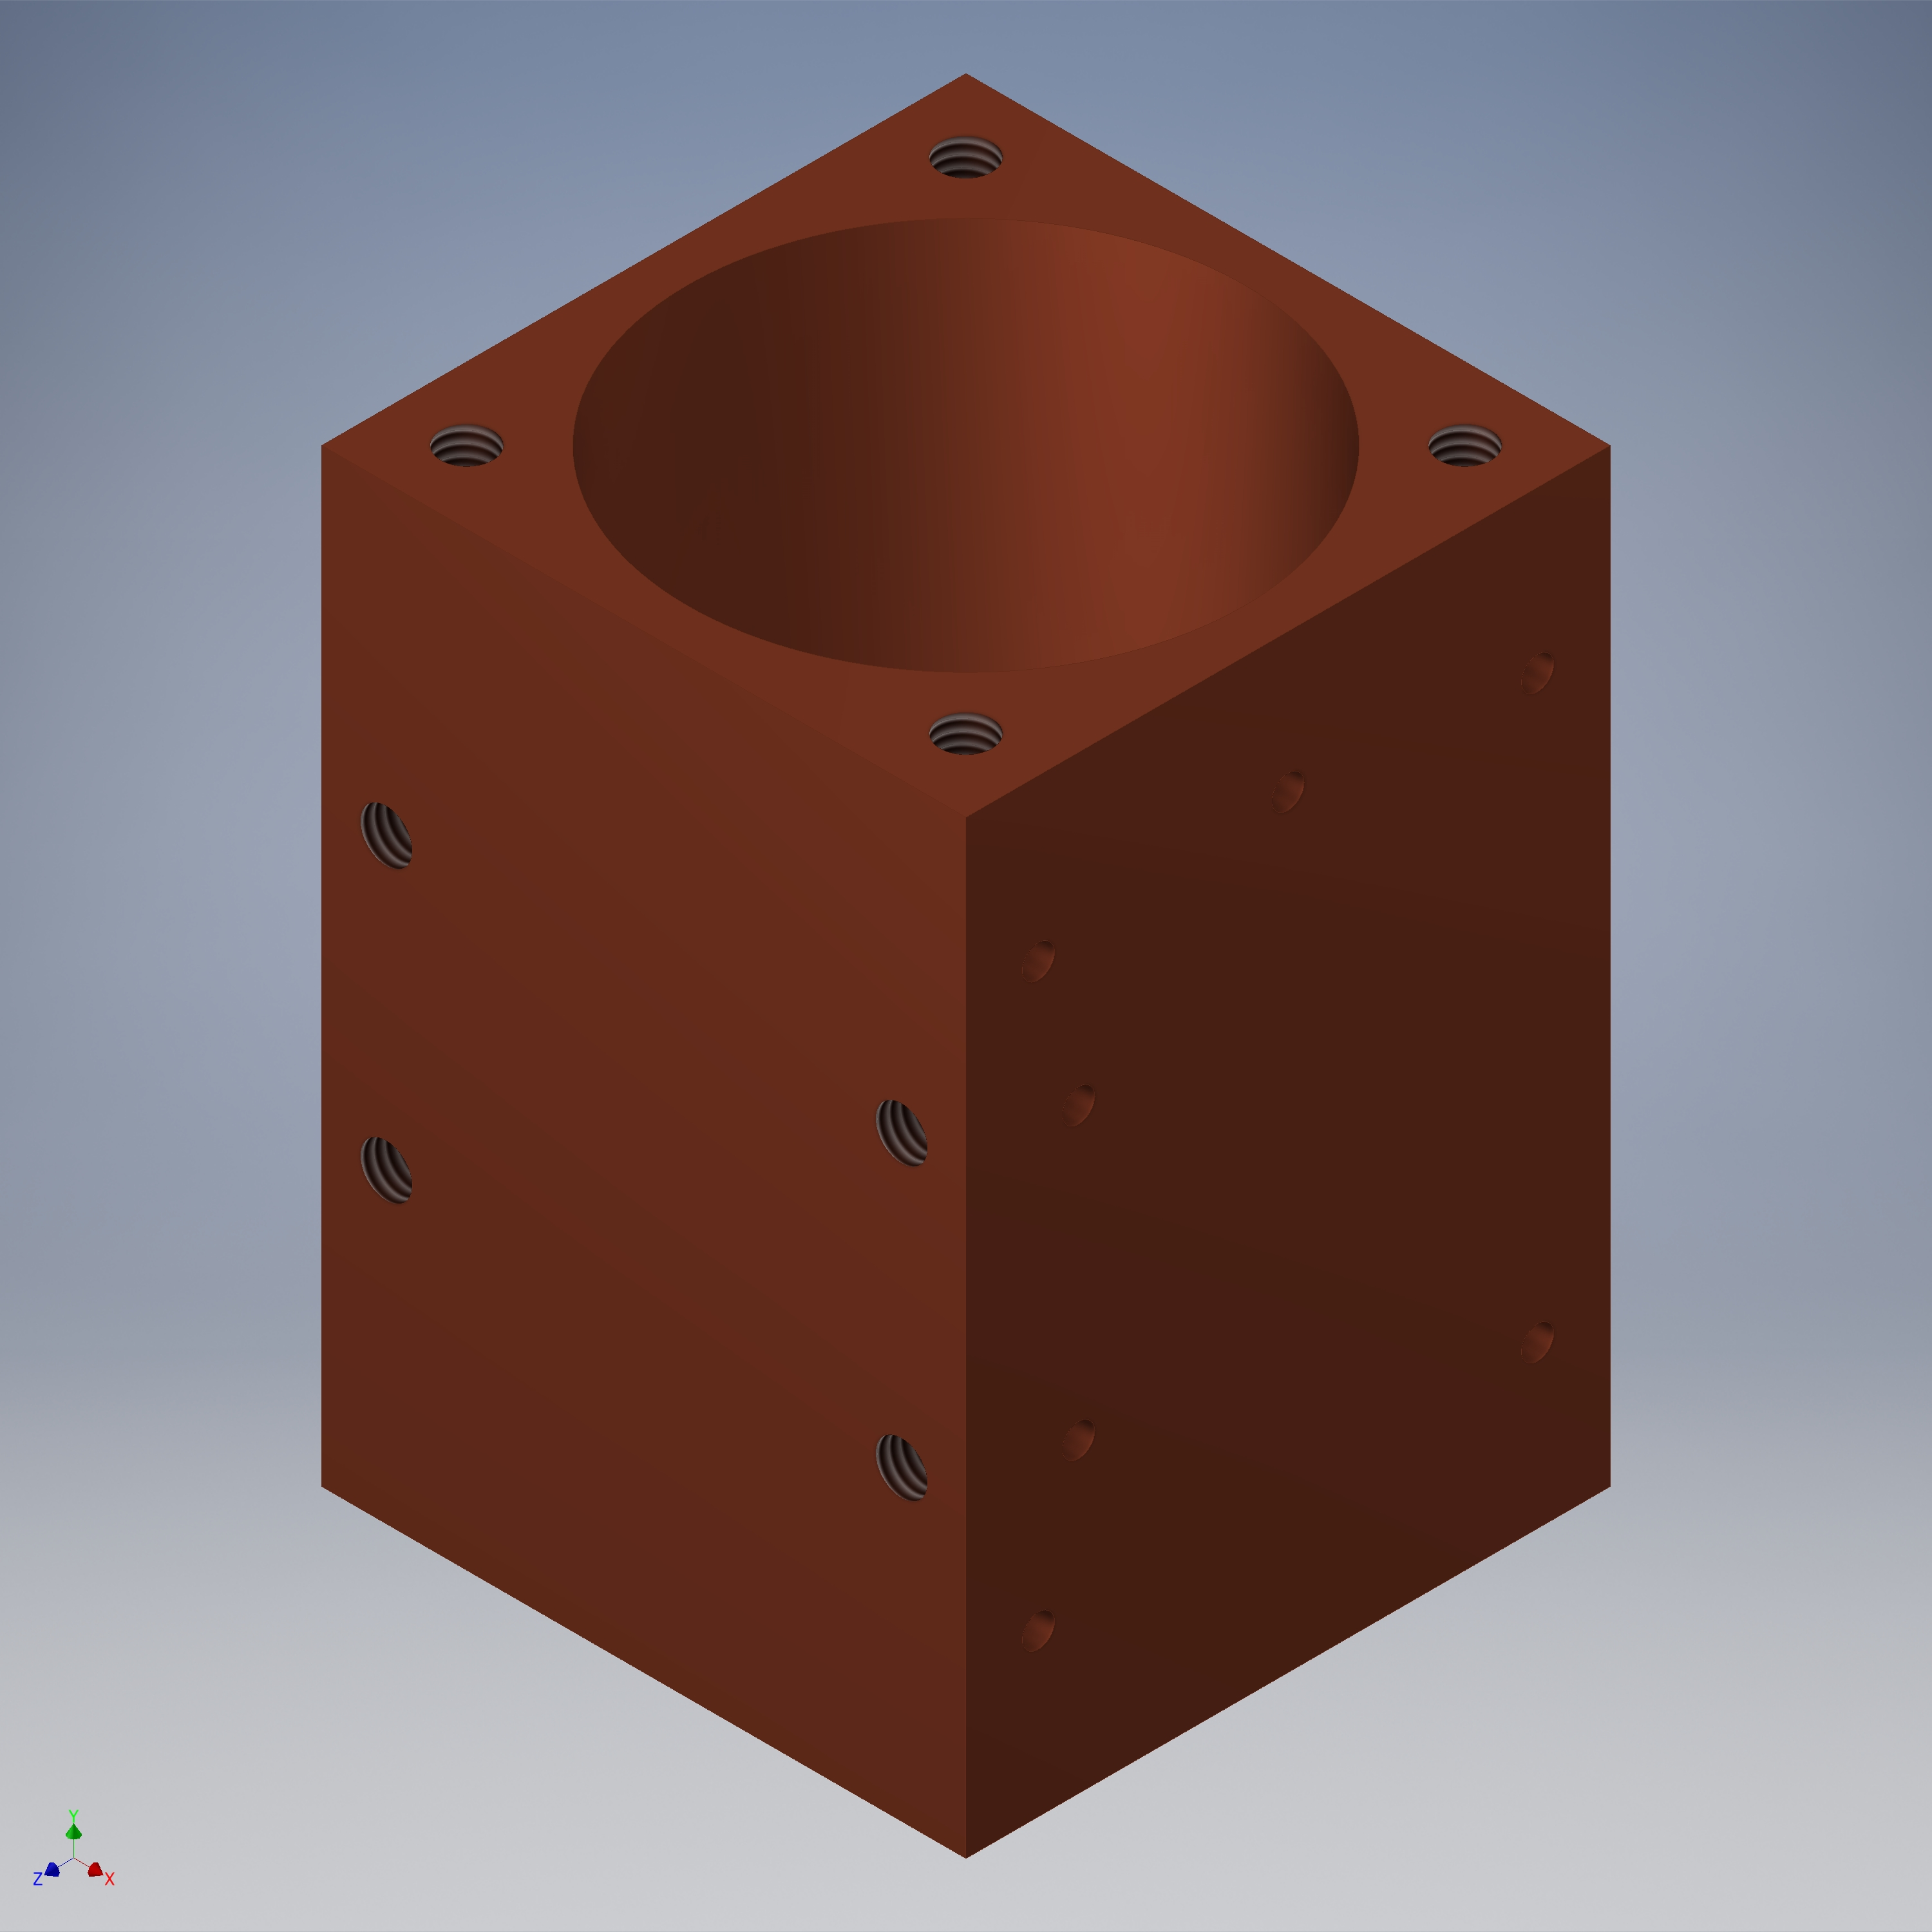
\includegraphics[width=\textwidth]{images/shield}
	\caption{3D model of a shield}
	\label{fig:shield}
\end{figure}

\clearpage
\subsection{Helix}
\label{subsection:helix}
Helix as displayed in the figure \ref{fig:helix} features:
\begin{itemize}
	\item end soldered to the shield (\ref{subsection:shield})
	\item end soldered to a SMA on the bottom cap (\ref{subsection:cap_bottom})
\end{itemize}

\begin{figure}[h]
	\centering
	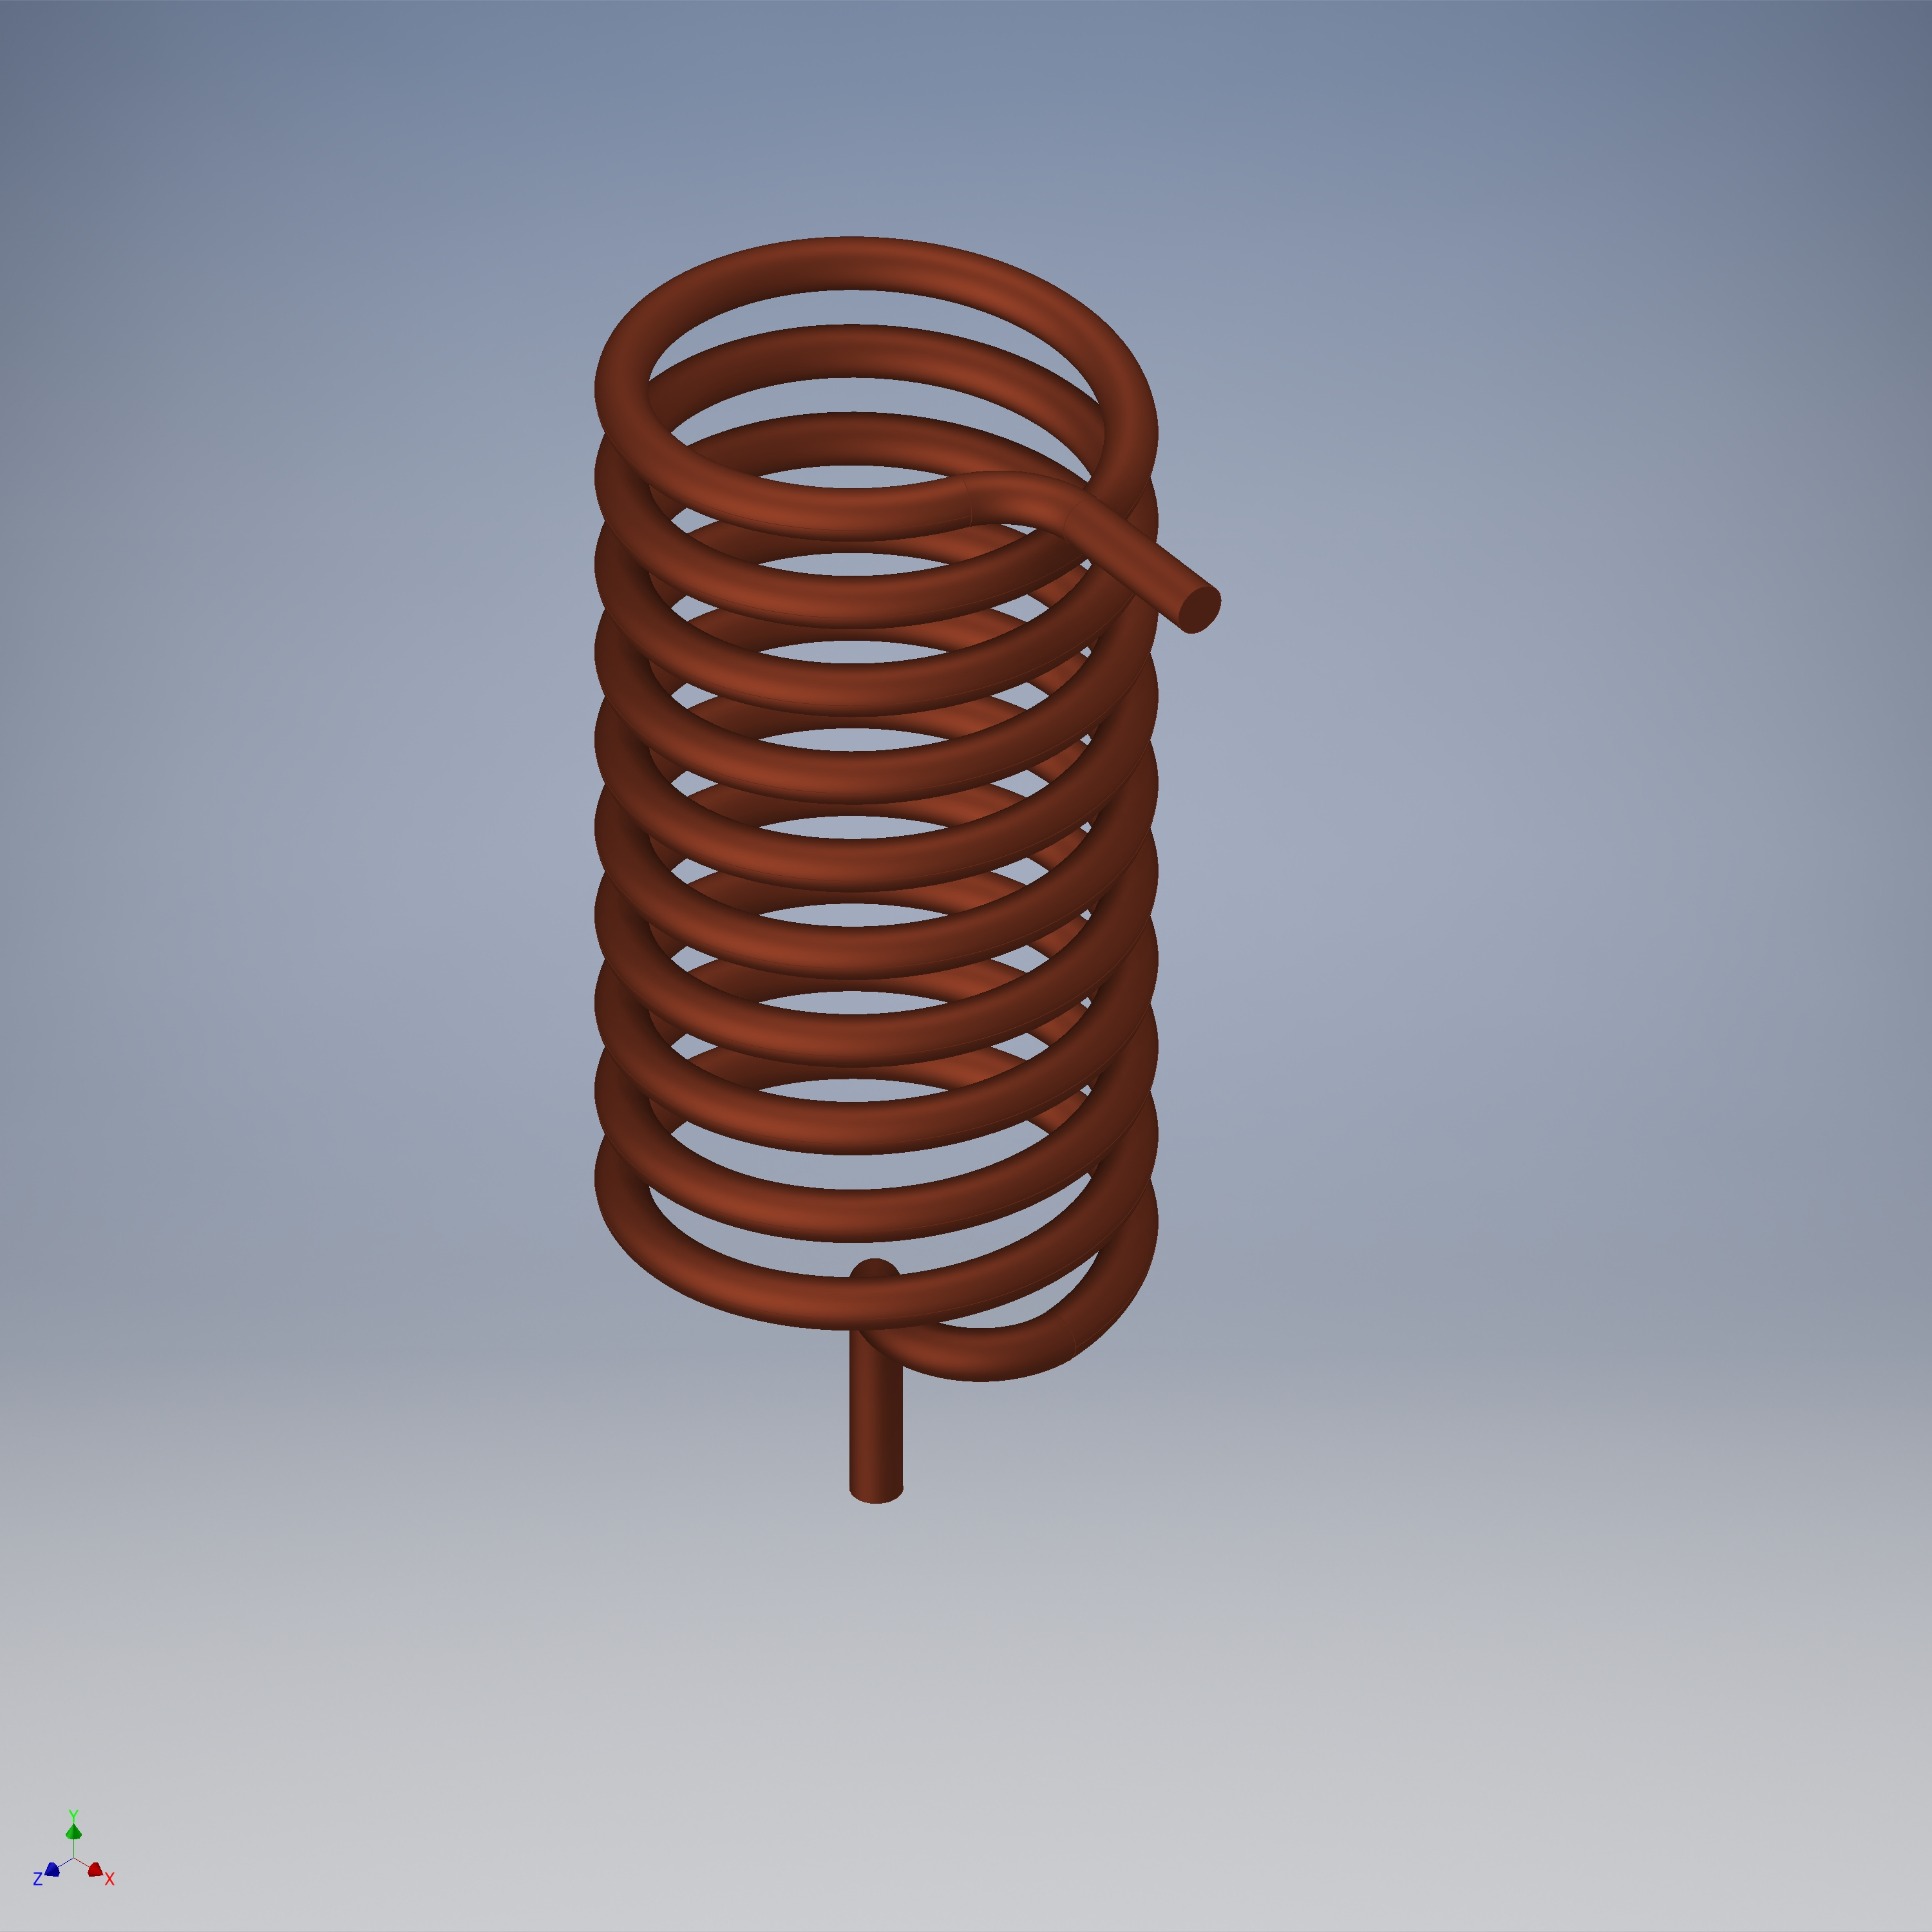
\includegraphics[width=\textwidth]{images/coil}
	\caption{3D model of a helix}
	\label{fig:helix}
\end{figure}

\clearpage
\subsection{Helix support}
\label{subsection:helix_support}
Since $d_0$ as specified in the table \ref{tbl:final_parameters} is smaller than recommended thickness of 5 mm the question of mechanical stability arises. In order to eliminate potential mechanical oscillations we introduce a helix support made of PEEK to be inserted inside of the helix (\ref{subsection:helix}). PEEK was selected as a cryogenic compatible insulator thus minimizing its influence on the helix's inductivity.

\begin{figure}[h]
	\centering
	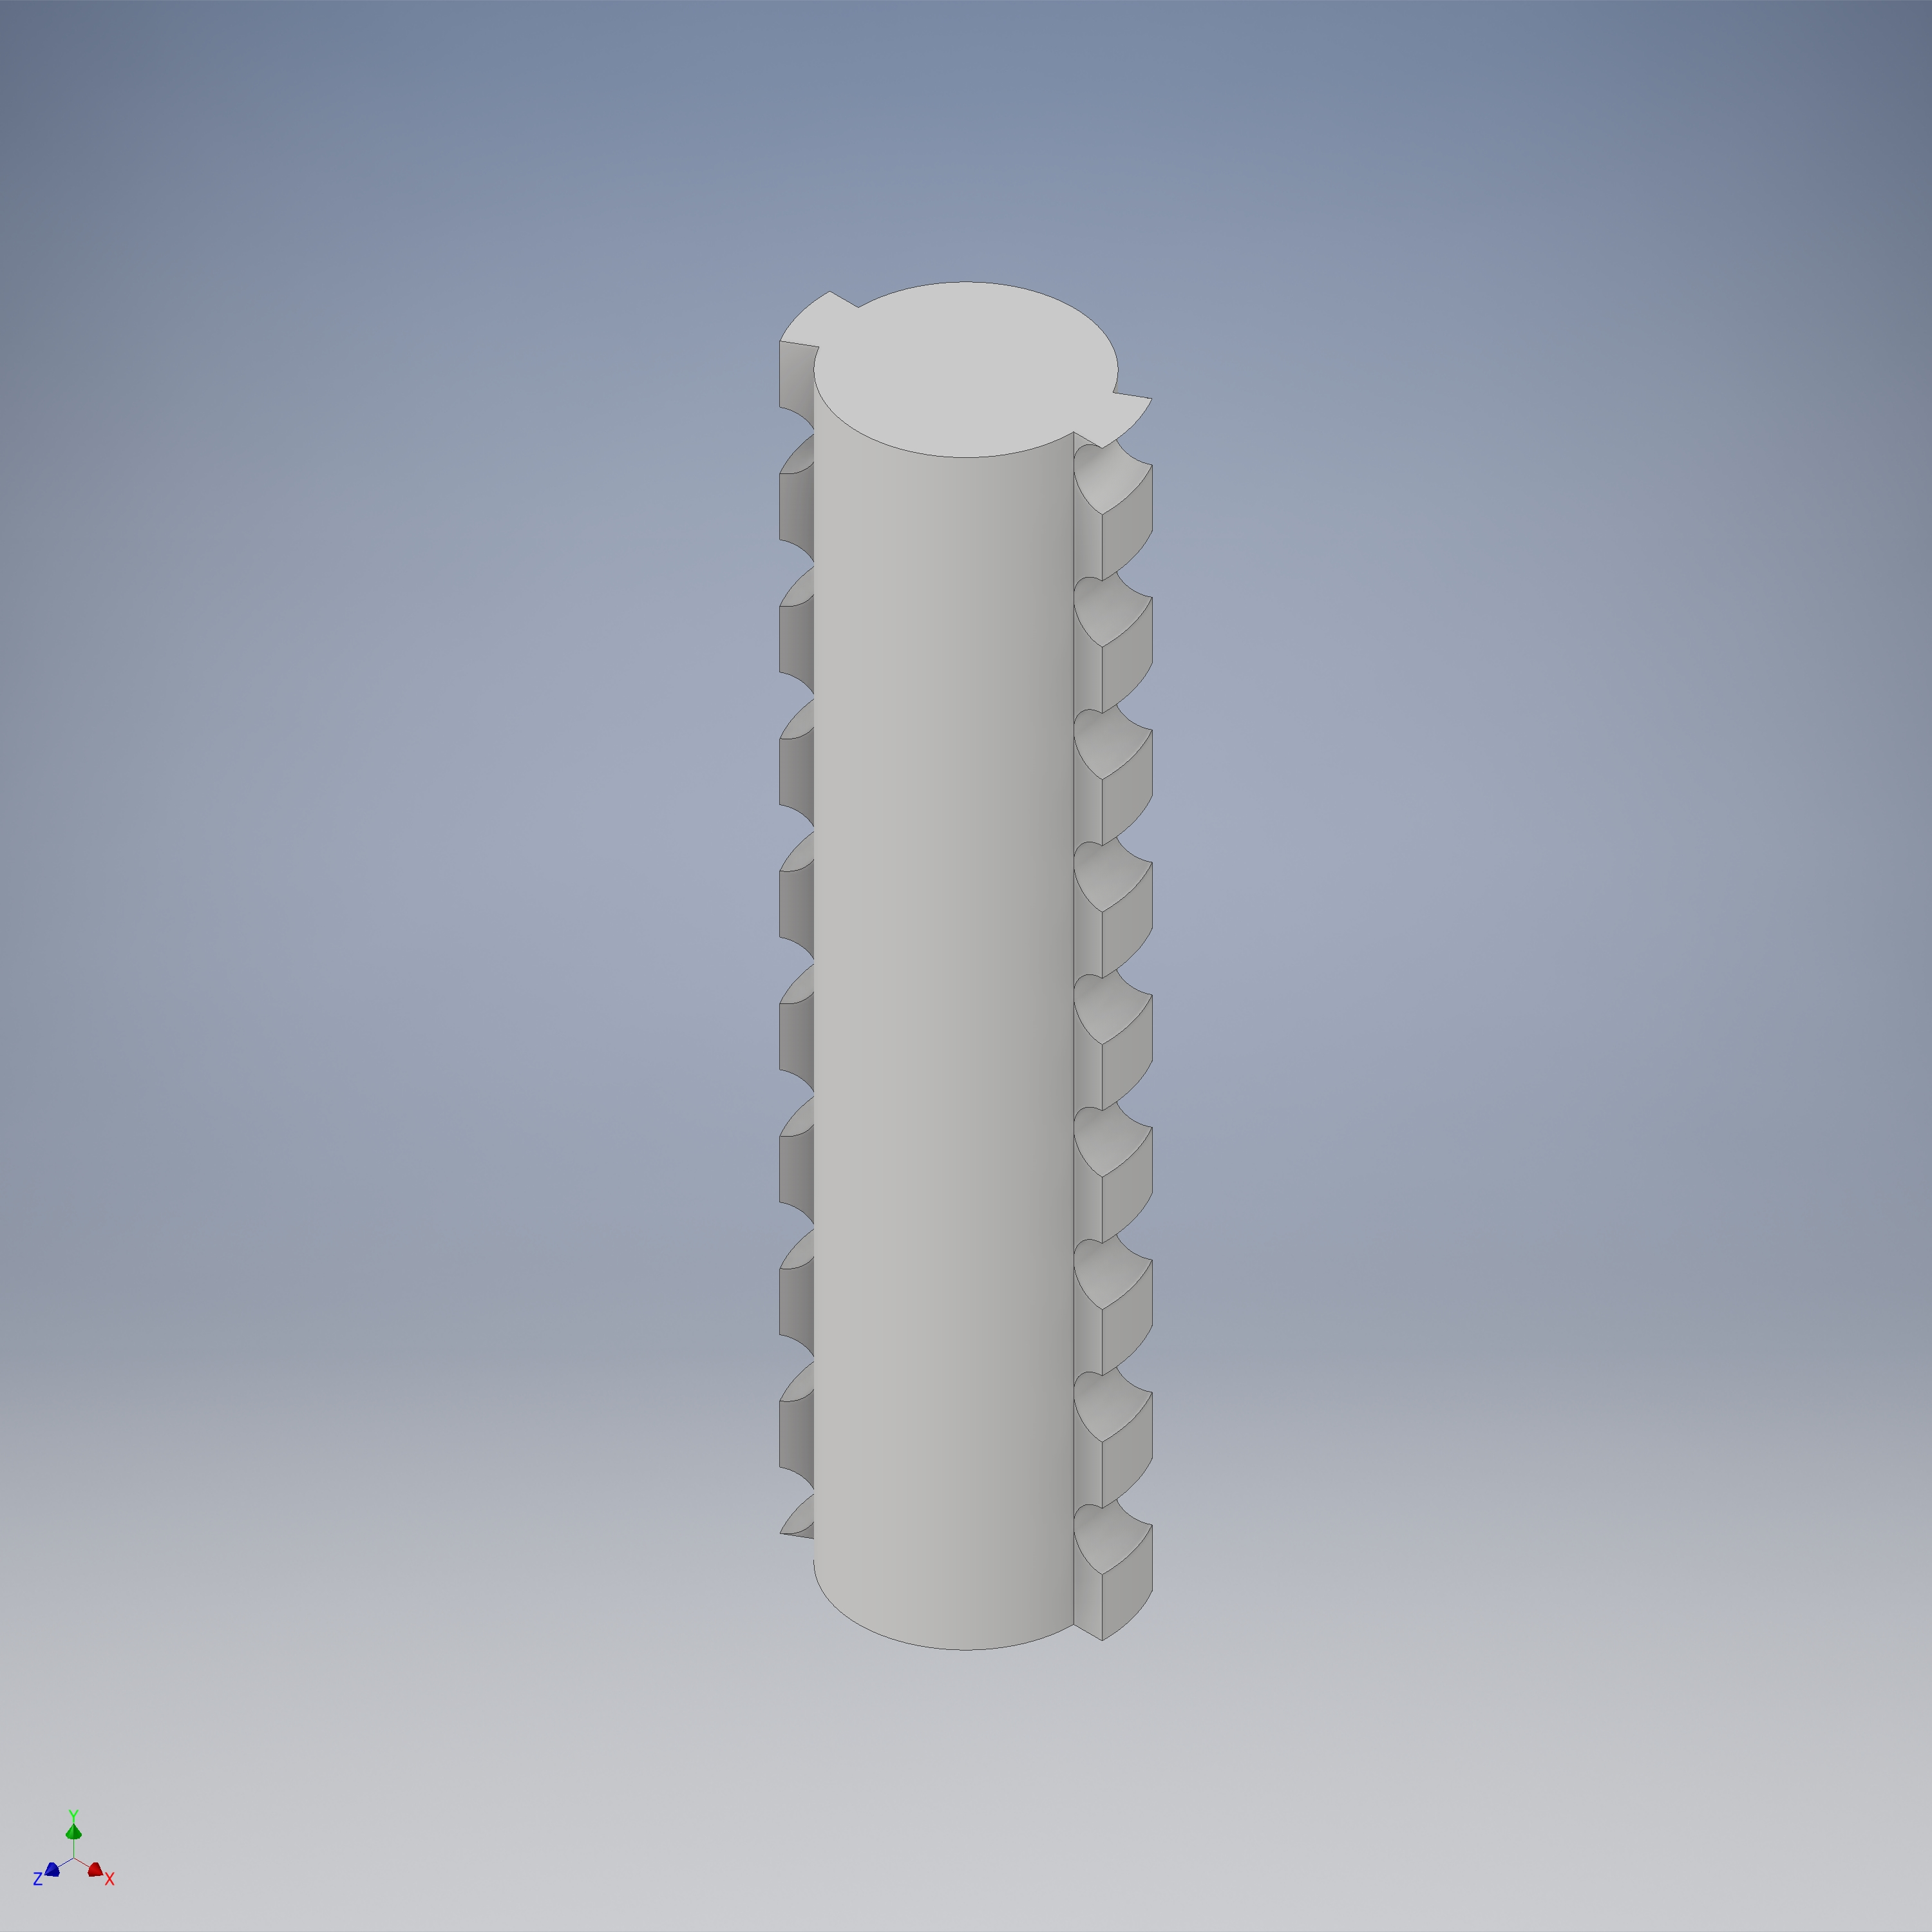
\includegraphics[width=\textwidth]{images/coil_support}
	\caption{3D model of a helix support}
	\label{fig:helix_support}
\end{figure}

\clearpage
\subsection{Top cap}
\label{subsection:cap_top}
Top cap as displayed in the figure \ref{fig:cap_top} features:
\begin{itemize}
	\item 4xM4 clearance holes to connect to the shield (\ref{subsection:shield})
	\item 4xM2 thread holes to connect to the top cap clamp (\ref{subsection:cap_top_clamp})
	\item tight hole for an antenna mount (\ref{subsection:antenna_mount})
	\item angular scale for an antenna mount (\ref{subsection:antenna_mount})
\end{itemize}

\begin{figure}[h]
	\centering
	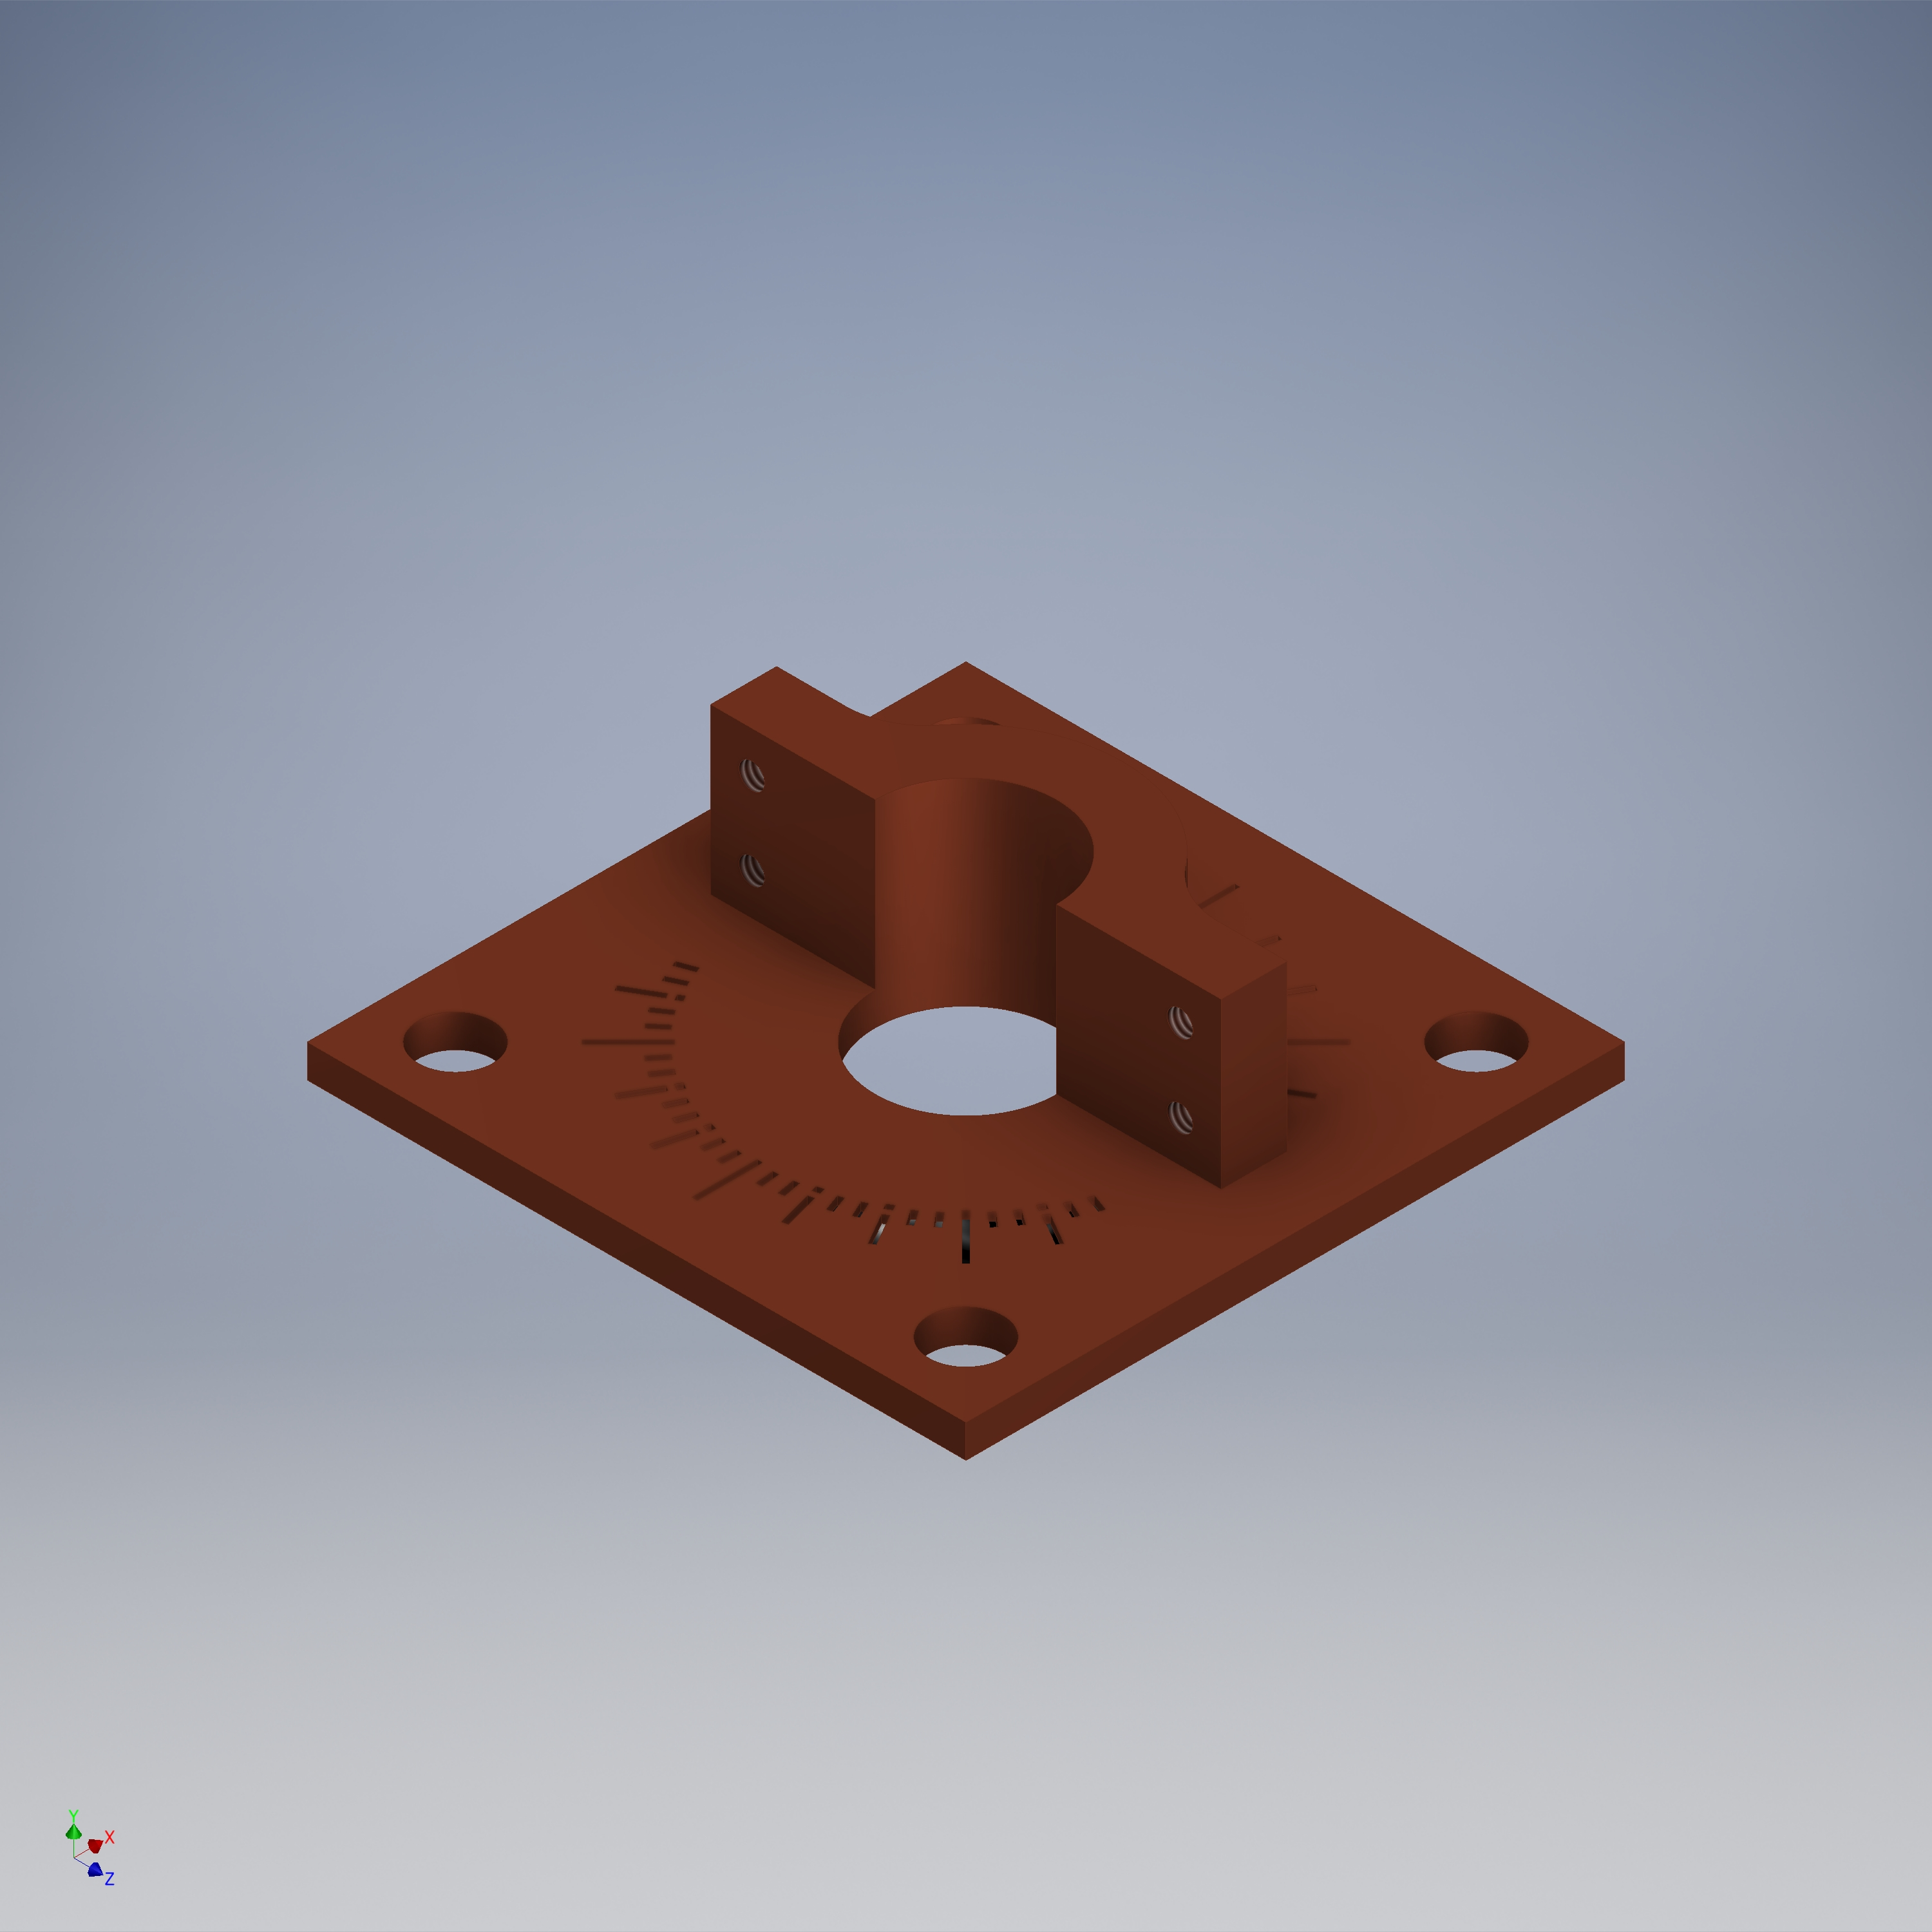
\includegraphics[width=\textwidth]{images/cap_top}
	\caption{3D model of a top cap}
	\label{fig:cap_top}
\end{figure}

\clearpage
\subsection{Top cap clamp}
\label{subsection:cap_top_clamp}
Top cap clamp as displayed in the figure \ref{fig:cap_top_clamp} features:
\begin{itemize}
	\item 4xM2 clearance holes to connect to the top cap (\ref{subsection:cap_top})
	\item truncated semicircle to clamp an antenna mount (\ref{subsection:antenna_mount})
\end{itemize}

\begin{figure}[h]
	\centering
	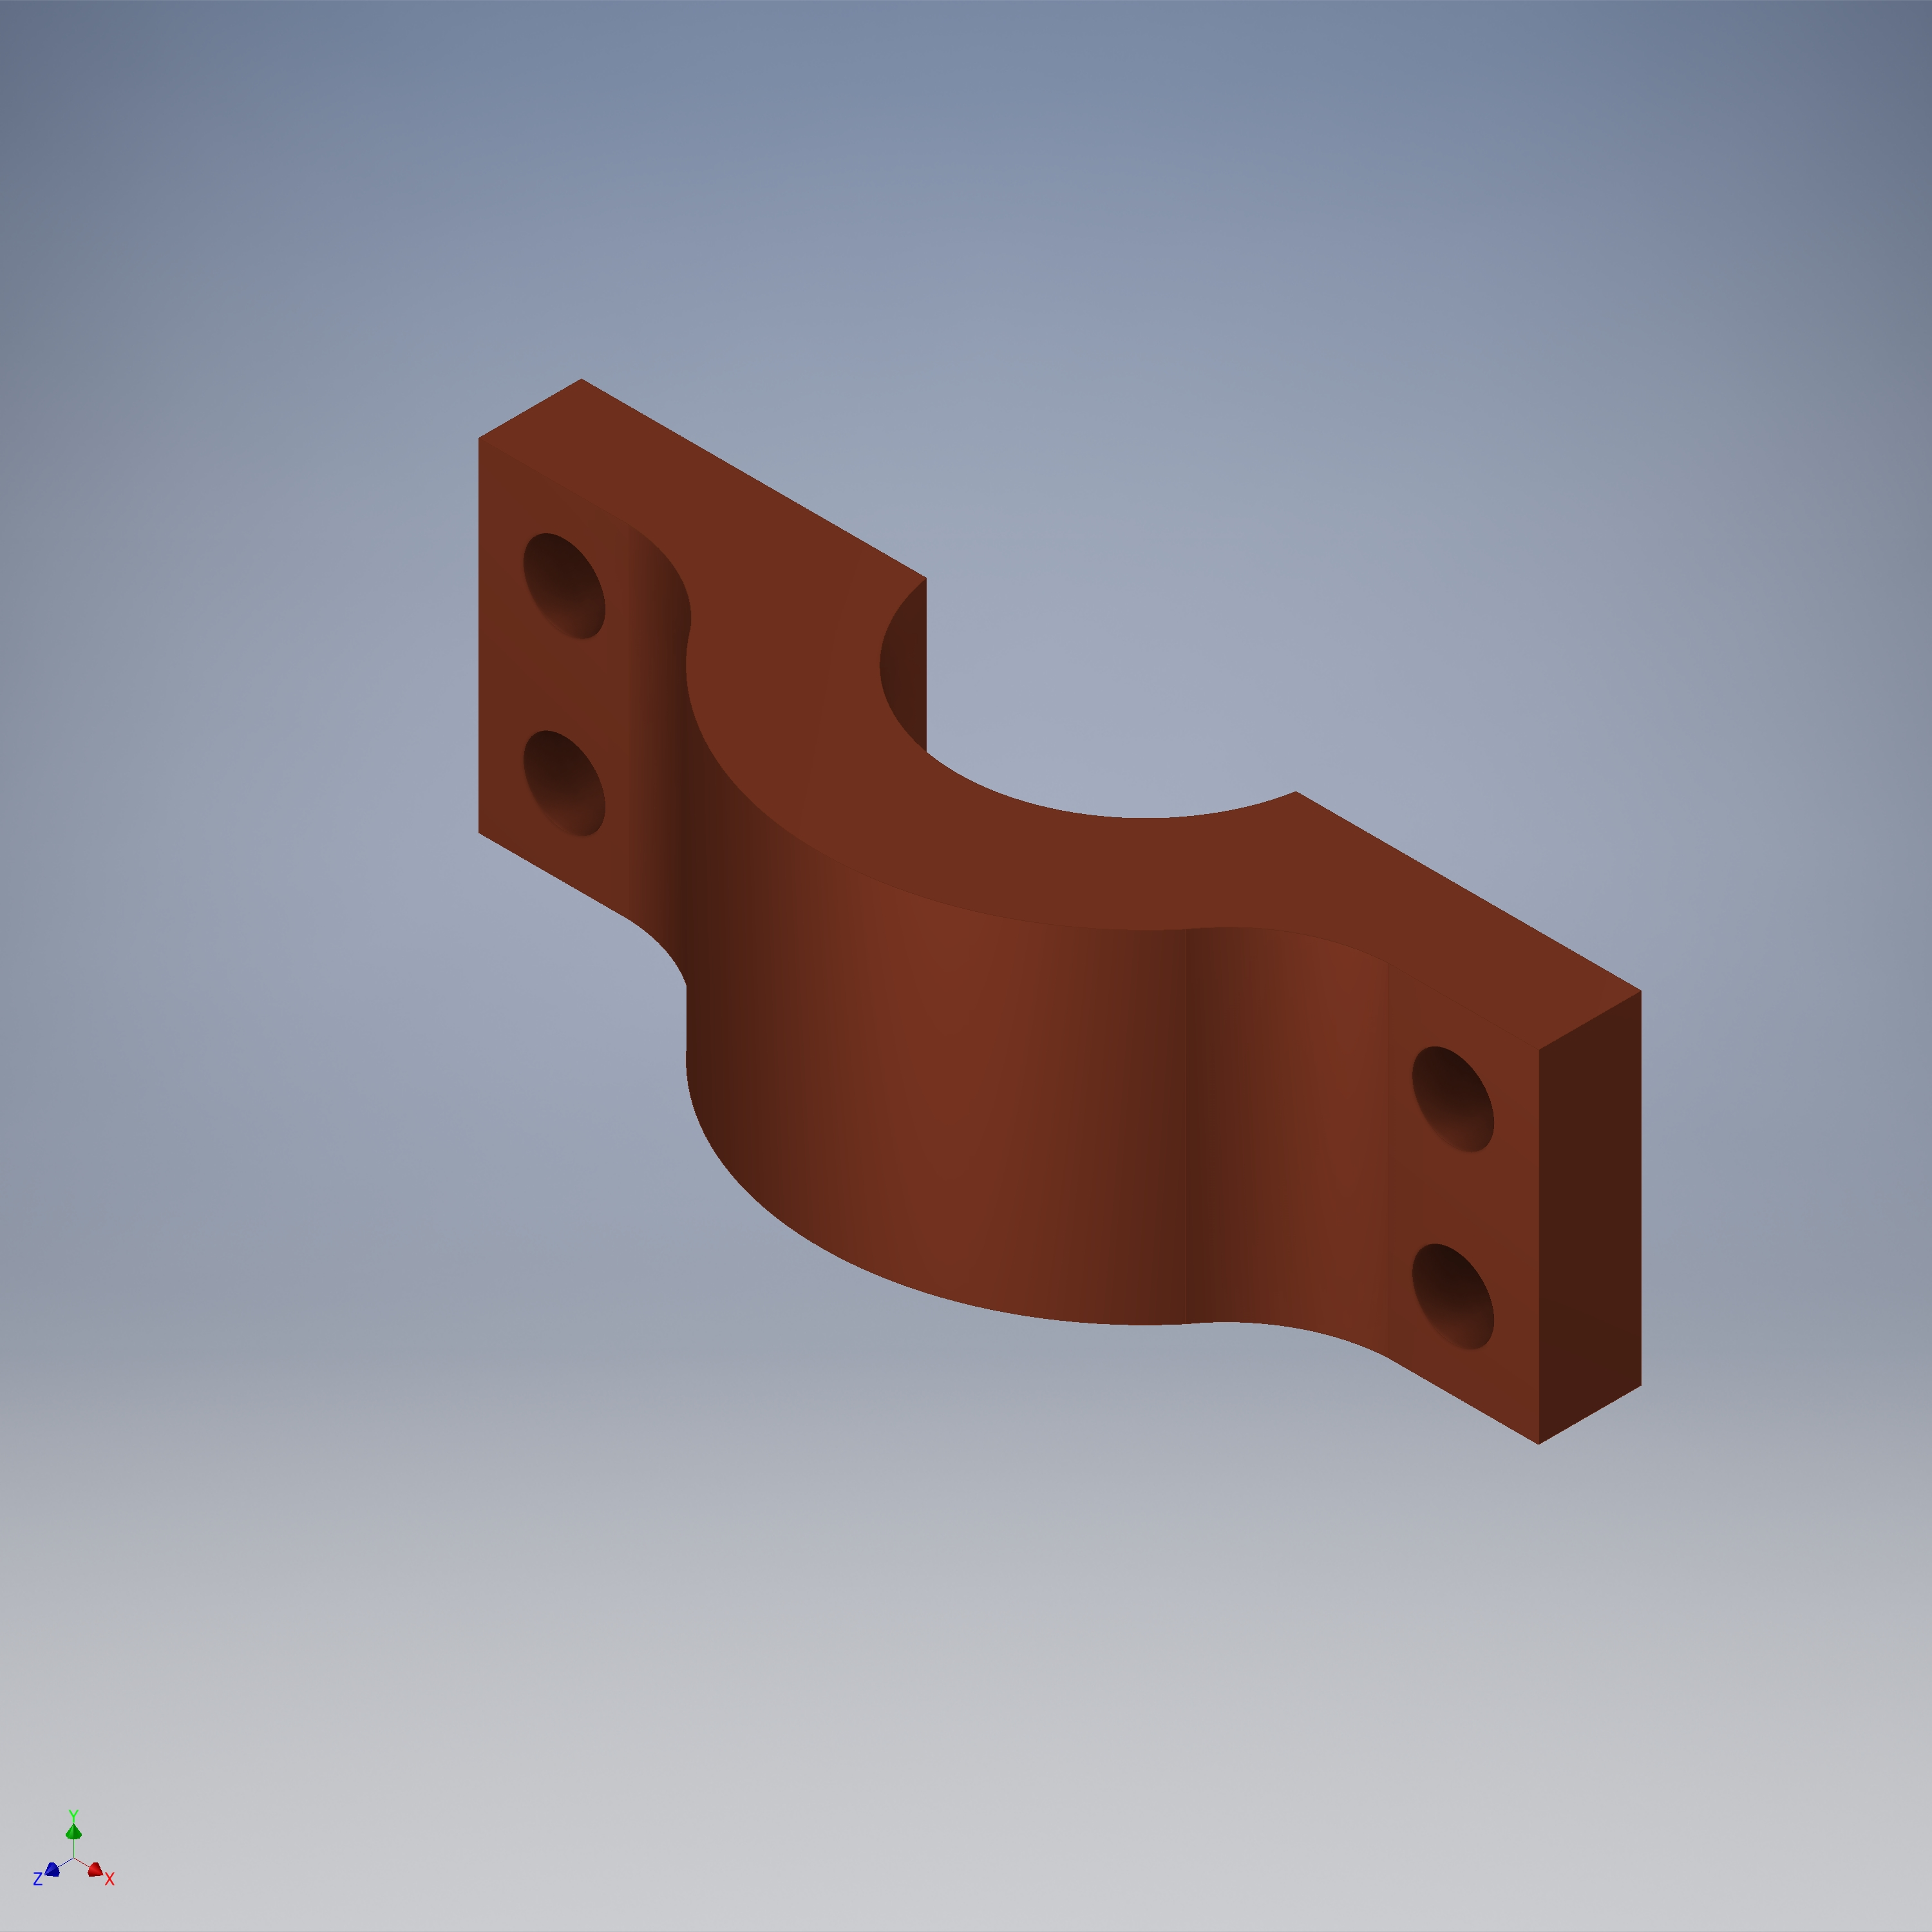
\includegraphics[width=\textwidth]{images/cap_top_movable}
	\caption{3D model of a top cap clamp}
	\label{fig:cap_top_clamp}
\end{figure}

\clearpage
\subsection{Antenna mount}
\label{subsection:antenna_mount}
Antenna mount as displayed in the figure \ref{fig:antenna_mount} features:
\begin{itemize}
	\item 2xM2 thread holes for a SMA connector for the antenna (\ref{subsection:antenna})
	\item hole for the antenna (\ref{subsection:antenna})
	\item cut for a precise usage of the angular scale on the top cap (\ref{subsection:cap_top})
	\item 1 mm period cuts to determine the distance to the top cap (\ref{subsection:cap_top})
\end{itemize}

\begin{figure}[h]
	\centering
	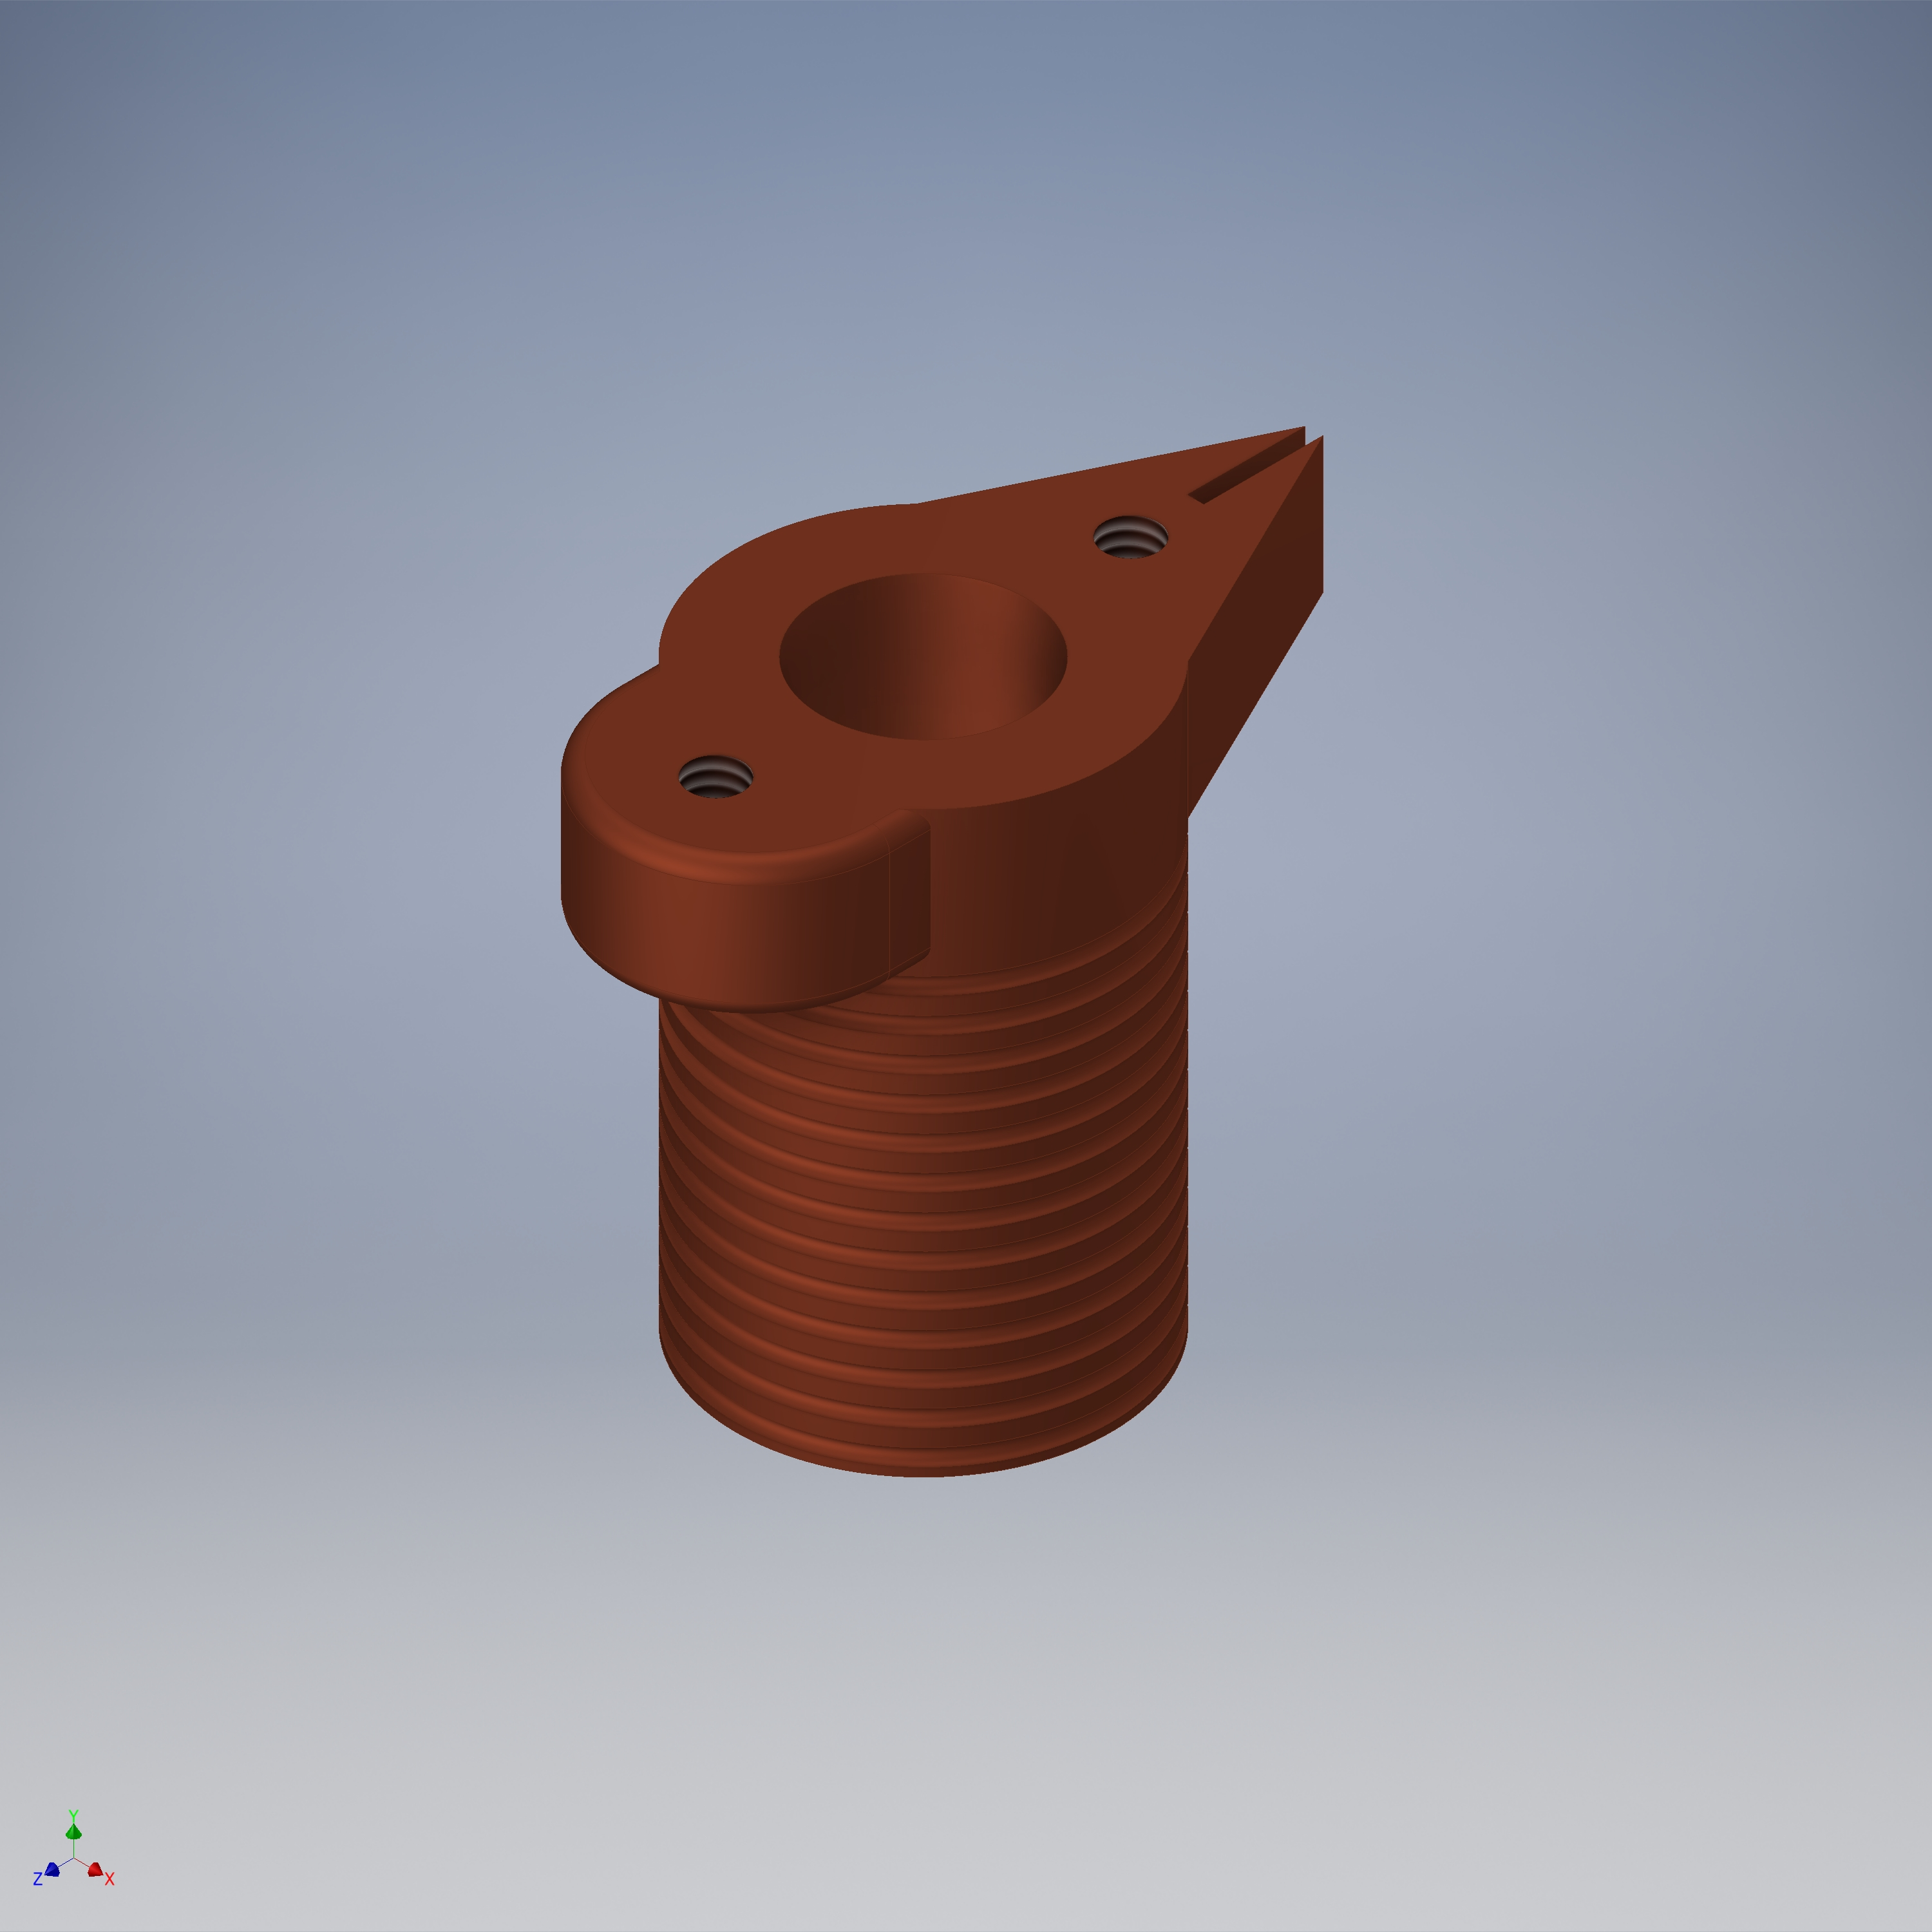
\includegraphics[width=\textwidth]{images/antenna_mount}
	\caption{3D model of an antenna mount}
	\label{fig:antenna_mount}
\end{figure}

\clearpage
\subsection{Antenna}
\label{subsection:antenna}
Antenna as displayed in the figure \ref{fig:antenna} features:
\begin{itemize}
	\item end connecting to a SMA on the antenna mount (\ref{subsection:antenna_mount})
	\item end soldered to the bottom of the antenna mount (\ref{subsection:antenna_mount})
	\item using empirical estimation from \cite{Siverns2012} a diameter of 11 mm was selected
\end{itemize}

\begin{figure}[h]
	\centering
	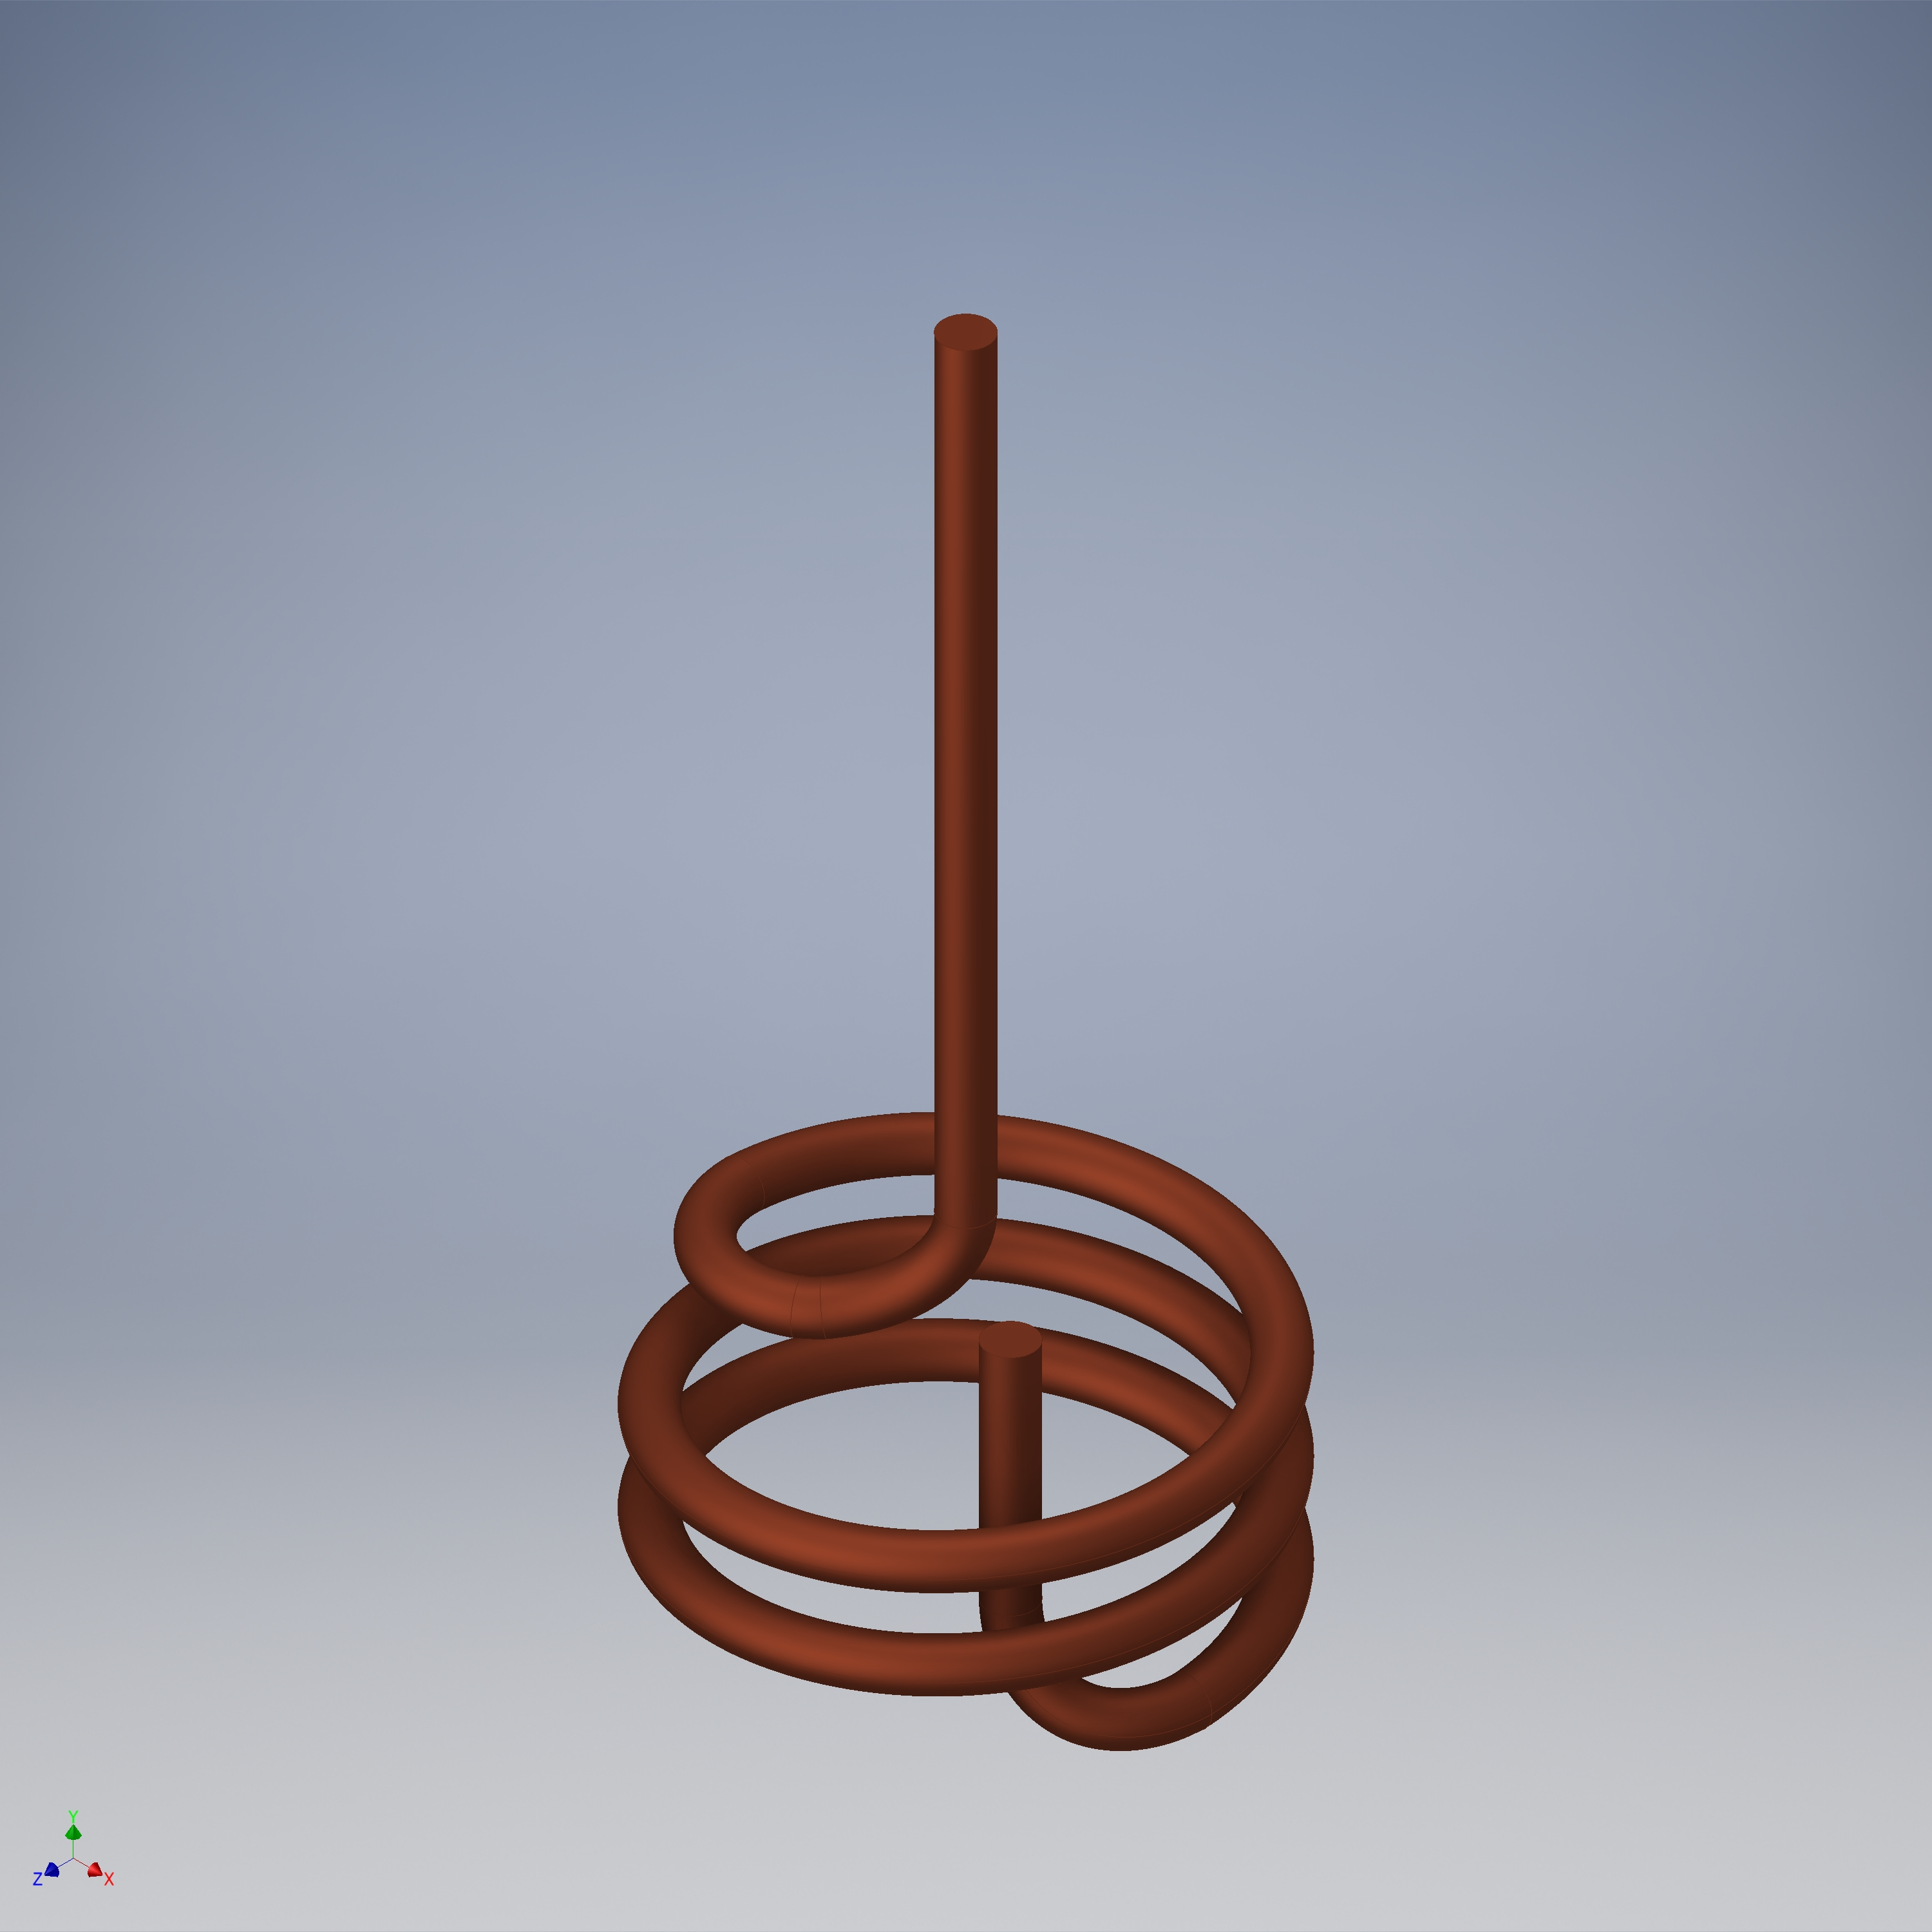
\includegraphics[width=\textwidth]{images/antenna}
	\caption{3D model of an antenna}
	\label{fig:antenna}
\end{figure}
